\documentclass[a4paper,14pt]{extarticle} %,twoside

%%% Проверка используемого TeX-движка %%%
\usepackage{iftex}
\newif\ifxetexorluatex   % определяем новый условный оператор (http://tex.stackexchange.com/a/47579/79756)
\ifXeTeX
    \xetexorluatextrue
\else
    \ifLuaTeX
        \xetexorluatextrue
    \else
        \xetexorluatexfalse
    \fi
\fi

%%% Поля и разметка страницы %%%
\usepackage{pdflscape}                              % Для включения альбомных страниц
\usepackage{geometry}                               % Для последующего задания полей

%%% Математические пакеты %%%
\usepackage{amsthm,amsfonts,amsmath,amssymb,amscd}  % Математические дополнения от AMS
\usepackage{mathtools}                              % Добавляет окружение multlined

%%%% Установки для размера шрифта 14 pt %%%%
%% Формирование переменных и констант для сравнения (один раз для всех подключаемых файлов)%%
%% должно располагаться до вызова пакета fontspec или polyglossia, потому что они сбивают его работу
\newlength{\curtextsize}
\newlength{\bigtextsize}
\setlength{\bigtextsize}{13.9pt}

\makeatletter
%\show\f@size                                       % неплохо для отслеживания, но вызывает стопорение процесса, если документ компилируется без команды  -interaction=nonstopmode 
\setlength{\curtextsize}{\f@size pt}
\makeatother

%%% Кодировки и шрифты %%%
\ifxetexorluatex
    \usepackage{polyglossia}                        % Поддержка многоязычности (fontspec подгружается автоматически)
\else
    \RequirePDFTeX                                  % tests for PDFTEX use and throws an error if a different engine is being used
   %%% Решение проблемы копирования текста в буфер кракозябрами
%    \input glyphtounicode.tex
%    \input glyphtounicode-cmr.tex %from pdfx package
%    \pdfgentounicode=1
    \usepackage{cmap}                               % Улучшенный поиск русских слов в полученном pdf-файле
    \defaulthyphenchar=127                          % Если стоит до fontenc, то переносы не впишутся в выделяемый текст при копировании его в буфер обмена
    \usepackage[T2A]{fontenc}                       % Поддержка русских букв
    \usepackage[utf8]{inputenc}                     % Кодировка utf8
    \usepackage[english, russian]{babel}            % Языки: русский, английский
    \IfFileExists{pscyr.sty}{\usepackage{pscyr}}{}  % Красивые русские шрифты
\fi

%%% Оформление абзацев %%%
\usepackage{indentfirst}                            % Красная строка

%%% Цвета %%%
\usepackage[dvipsnames,usenames]{color}
\usepackage{colortbl}
%\usepackage[dvipsnames, table, hyperref, cmyk]{xcolor} % Вероятно, более новый вариант, вместо предыдущих двух строк. Конвертация всех цветов в cmyk заложена как удовлетворение возможного требования типографий. Возможно конвертирование и в rgb.

%%% Таблицы %%%
\usepackage{longtable}                              % Длинные таблицы
\usepackage{multirow,makecell,array}                % Улучшенное форматирование таблиц
\usepackage{booktabs}                               % Возможность оформления таблиц в классическом книжном стиле (при правильном использовании не противоречит ГОСТ)

%%% Общее форматирование
\usepackage{soulutf8}                               % Поддержка переносоустойчивых подчёркиваний и зачёркиваний
\usepackage{icomma}                                 % Запятая в десятичных дробях


%%% Гиперссылки %%%
\usepackage{hyperref}

%%% Изображения %%%
\usepackage{graphicx}                               % Подключаем пакет работы с графикой

%%% Списки %%%
\usepackage{enumitem}

%%% Подписи %%%
\usepackage{caption}                                % Для управления подписями (рисунков и таблиц) % Может управлять номерами рисунков и таблиц с caption %Иногда может управлять заголовками в списках рисунков и таблиц
\usepackage{subcaption}                             % Работа с подрисунками и подобным

%%% Интервалы %%%
\usepackage[onehalfspacing]{setspace}               % Опция запуска пакета правит не только интервалы в обычном тексте, но и формульные

%%% Счётчики %%%
\usepackage[figure,table]{totalcount}               % Счётчик рисунков и таблиц
\usepackage{totcount}                               % Пакет создания счётчиков на основе последнего номера подсчитываемого элемента (может требовать дважды компилировать документ)
\usepackage{totpages}                               % Счётчик страниц, совместимый с hyperref (ссылается на номер последней страницы). Желательно ставить последним пакетом в преамбуле

%%% Продвинутое управление групповыми ссылками (пока только формулами) %%%
\ifxetexorluatex
    \usepackage{cleveref}                           % cleveref корректно считывает язык из настроек polyglossia
\else
    \usepackage[russian]{cleveref}                  % cleveref имеет сложности со считыванием языка из babel. Такое решение русификации вывода выбрано вместо определения в documentclass из опасности что-то лишнее передать во все остальные пакеты, включая библиографию.
\fi
\creflabelformat{equation}{#2#1#3}                  % Формат по умолчанию ставил круглые скобки вокруг каждого номера ссылки, теперь просто номера ссылок без какого-либо дополнительного оформления

%\usepackage[caption=false]{subfig}
\RequirePackage{xspace}
  % Пакеты общие для диссертации и автореферата
%%% Опционально %%%
% Следующий пакет может быть полезен, если надо ужать текст, чтобы сам текст не править, но чтобы места он занимал поменьше
%\usepackage{savetrees}

% Этот пакет может быть полезен для печати текста брошюрой
%\usepackage[print]{booklet}         % Пакеты для автореферата
\usepackage{tabularx,tabulary}  %таблицы с автоматически подбирающейся шириной столбцов

% Листинги с исходным кодом программ
\usepackage{fancyvrb}
\usepackage{listings}

% Плавающие окружения. во многом лучше пакета float
\usepackage{floatrow}

% Русская традиция начертания греческих букв
%\usepackage{upgreek} % прямые греческие ради русской традиции        % Пакеты для специфических пользовательских задач

% Новые переменные, которые могут использоваться во всём проекте
\newcommand{\authorbibtitle}{Публикации автора по теме диссертации}
\newcommand{\fullbibtitle}{Список литературы} % (ГОСТ Р 7.0.11-2011, 4)

\newcommand{\ccbar}{\ensuremath{c\overline{c}}\xspace}
\newcommand{\nb}{\ensuremath{~\text{нб}}\xspace}
\newcommand{\pn}{\ensuremath{P^0}\xspace}
\newcommand{\dn}{\ensuremath{D^0}\xspace}
\newcommand{\bn}{\ensuremath{B^0}\xspace}
\newcommand{\hn}{\ensuremath{h^0}\xspace}
\newcommand{\dbar}{\ensuremath{\overline{D}}\xspace}
\newcommand{\pbar}{\ensuremath{\overline{P}}\xspace}
\newcommand{\bbar}{\ensuremath{\overline{B}}\xspace}
\newcommand{\fbar}{\ensuremath{\overline{f}}\xspace}
\newcommand{\qbar}{\ensuremath{\overline{q}}\xspace}
\newcommand{\bbbar}{\ensuremath{B\bbar}\xspace}
\newcommand{\qqbar}{\ensuremath{q\qbar}\xspace}
\newcommand{\ddbar}{\ensuremath{D\dbar}\xspace}
\newcommand{\dnbar}{\ensuremath{\dbar{}^0}\xspace}
\newcommand{\bnbar}{\ensuremath{\bbar{}^0}\xspace}
\newcommand{\pnbar}{\ensuremath{\pbar{}^0}\xspace}
\newcommand{\dstn}{\ensuremath{D^{*0}}\xspace}
\newcommand{\dstp}{\ensuremath{D^{*+}}\xspace}
\newcommand{\dstm}{\ensuremath{D^{*-}}\xspace}
\newcommand{\dstarn}{\ensuremath{D^{(*)0}}\xspace}
\newcommand{\dstnbar}{\ensuremath{\dbar{}^{*0}}\xspace}
\newcommand{\dstarnbar}{\ensuremath{\dbar{}^{(*)0}}\xspace}
\newcommand{\ks}{\ensuremath{K_S^0}\xspace}
\newcommand{\pip}{\ensuremath{\pi^+}\xspace}
\newcommand{\pim}{\ensuremath{\pi^-}\xspace}
\newcommand{\pin}{\ensuremath{\pi^0}\xspace}
\newcommand{\kstopipi}{\ensuremath{\ks\to\pip\pim}\xspace}
\newcommand{\cms}{\ensuremath{\textrm{СЦМ}}\xspace}


\newcommand{\prm}{\ensuremath{{}^{\prime}}\xspace}
\newcommand{\pprm}{\ensuremath{{}^{\prime\prime}}\xspace}
\newcommand{\ppprm}{\ensuremath{{}^{\prime\prime\prime}}\xspace}

\newcommand{\aphi}{\ensuremath{\alpha}\xspace}
\newcommand{\pphi}{\ensuremath{\beta}\xspace}
\newcommand{\gphi}{\ensuremath{\gamma}\xspace}
\newcommand{\sindbeta}{\ensuremath{\sin{2\pphi}}\xspace}
\newcommand{\cosdbeta}{\ensuremath{\cos{2\pphi}}\xspace}
%\newcommand{\pphib}{\ensuremath{\varphi_2}\xspace}
%\newcommand{\pphig}{\ensuremath{\varphi_3}\xspace}
\newcommand{\pphieff}{\ensuremath{\pphi_{\mathrm{eff}}}\xspace}
\newcommand{\sindbetaeff}{\ensuremath{\sin{2\pphieff}}\xspace}

\newcommand{\gamb}{\ensuremath{\Gamma_B}\xspace}
\newcommand{\gamt}{\ensuremath{\Gamma t}\xspace}
\newcommand{\gamdt}{\ensuremath{\Gamma_Dt}\xspace}
\newcommand{\gambt}{\ensuremath{\gamb t}\xspace}
\newcommand{\oxdydtsq}{\ensuremath{\mco\left((\gamdt)^2(x_D+y_D)^2\right)}\xspace}
\newcommand{\oxdydsq}{\ensuremath{\mco\left(x_D+y_D\right)^2}\xspace}
\newcommand{\orbxdyd}{\ensuremath{\mco\lbr\rb\lbr x_D+y_D\rbr\rbr}\xspace}
\newcommand{\emdgd}{\ensuremath{e^{-im_Dt-\frac{\gamdt}{2}}}\xspace}
\newcommand{\embgb}{\ensuremath{e^{-im_Bt-\frac{\gambt}{2}}}\xspace}
\newcommand{\emg}{\ensuremath{e^{-imt-\frac{\gamt}{2}}}\xspace}

\newcommand{\lbr}{\ensuremath{\left(}}
\newcommand{\rbr}{\ensuremath{\right)}}

\newcommand{\rcp}{\ensuremath{r_{\cpconj}}}
\newcommand{\alcp}{\ensuremath{\alpha_{\cpconj}}}
    
\newcommand{\bdk}{\ensuremath{B^{\pm}\to D K^{\pm}}\xspace}
\newcommand{\bdkp}{\ensuremath{B^+\to D K^+}\xspace}
\newcommand{\bdnkp}{\ensuremath{B^+\to\dn K^+}\xspace}
\newcommand{\bdbkp}{\ensuremath{B^+\to\dnbar K^+}\xspace}
\newcommand{\bdnkm}{\ensuremath{B^-\to\dn K^-}\xspace}
\newcommand{\bdbkm}{\ensuremath{B^-\to\dnbar K^-}\xspace}
\newcommand{\bdkm}{\ensuremath{B^-\to D K^-}\xspace}
\newcommand{\bdcpk}{\ensuremath{B^+\to D_{\cpconj} K^+}\xspace}

\newcommand{\delf}{\ensuremath{\Delta\delta_f}\xspace}
\newcommand{\deld}{\ensuremath{\Delta\delta_D}\xspace}
\newcommand{\delb}{\ensuremath{\Delta\delta_B}\xspace}
\newcommand{\rb}{\ensuremath{r_B}\xspace}
\newcommand{\rd}{\ensuremath{r_D}\xspace}
\newcommand{\mbc}{\ensuremath{M_{\mathrm{bc}}}\xspace}
\newcommand{\de}{\ensuremath{\Delta E}\xspace}
\newcommand{\dm}{\ensuremath{\Delta m}\xspace}
\newcommand{\dg}{\ensuremath{\Delta\Gamma}\xspace}
\newcommand{\debk}{\ensuremath{\left(\Delta E\right)}\xspace}

\newcommand{\br}{\ensuremath{\mathcal{B}}\xspace}
\newcommand{\dkpi}{\ensuremath{D\to K^+\pi^-}\xspace}
\newcommand{\dkpbar}{\ensuremath{D\to K^-\pi^+}\xspace}

\newcommand{\dd}{\ensuremath{\mathrm{d}}\xspace}
\newcommand{\ddlz}{\dd\mpsq\dd\mmsq}

\newcommand{\vckm}{\ensuremath{V_{\mathrm{CKM}}}\xspace}
\newcommand{\cabang}{\ensuremath{\theta_{\mathrm{C}}}\xspace}

\newcommand{\kspp}{\ensuremath{\ks\pi^+\pi^-}\xspace}
\newcommand{\kppn}{\ensuremath{K^-\pi^+\pin}\xspace}
\newcommand{\dkpp}{\ensuremath{D\to\ks\pi^+\pi^-}\xspace}
\newcommand{\dnkpp}{\ensuremath{\dn\to\ks\pi^+\pi^-}\xspace}
\newcommand{\dbkpp}{\ensuremath{\dnbar\to\ks\pi^+\pi^-}\xspace}
\newcommand{\dkspp}{\ensuremath{\dn\to\ks\pi^+\pi^-}\xspace}

\newcommand{\bpdrho}{\ensuremath{B^+\to\dnbar\rho^+}\xspace}
\newcommand{\bpdstarrho}{\ensuremath{B^+\to\dstarnbar\rho^+}\xspace}
\newcommand{\bpdstarpi}{\ensuremath{B^+\to\dstarnbar\pi^+}\xspace}
\newcommand{\bpdstph}{\ensuremath{B^+\to\dstp\hn}\xspace}

\newcommand{\bmdrho}{\ensuremath{B^-\to\dn\rho^-}\xspace}
\newcommand{\bmdstpi}{\ensuremath{B^-\to\dstm\pin}\xspace}
\newcommand{\bmdstrho}{\ensuremath{B^-\to\dstn\rho^-}\xspace}
\newcommand{\bmdstarrho}{\ensuremath{B^-\to\dstarn\rho^-}\xspace}
\newcommand{\bmdstph}{\ensuremath{B^-\to\dstm\hn}\xspace}

\newcommand{\etap}{\ensuremath{\eta^{\prime}}\xspace}

\newcommand{\bbdsth}{\ensuremath{\bnbar\to\dstarn\hn}\xspace}
\newcommand{\bdh}{\ensuremath{\bn\to\dnbar\hn}\xspace}
\newcommand{\bdnh}{\ensuremath{\bn\to\dn\hn}\xspace}
\newcommand{\bdsth}{\ensuremath{\bn\to\dstarnbar\hn}\xspace}
\newcommand{\bdstarh}{\ensuremath{\bn\to\dstnbar\hn}\xspace}
\newcommand{\bdpi}{\ensuremath{\bn\to\dnbar\pin}\xspace}
\newcommand{\bdeta}{\ensuremath{\bn\to\dnbar\eta}\xspace}
%\newcommand{\bdetagg}{\ensuremath{\bn\to\dnbar\eta_{\gamma\gamma}}\xspace}
\newcommand{\bdetagg}{\ensuremath{\bn\to\dnbar[\gamma\gamma]_{\eta}}\xspace}
\newcommand{\bdstaretagg}{\ensuremath{\bn\to\dstarnbar[\gamma\gamma]_{\eta}}\xspace}
\newcommand{\bdetap}{\ensuremath{\bn\to\dnbar\etap}\xspace}
\newcommand{\bdetappp}{\ensuremath{\bn\to\dnbar[\pi^+\pi^-\pi^0]_{\eta}}\xspace}
\newcommand{\bdomega}{\ensuremath{\bn\to\dnbar\omega}\xspace}
\newcommand{\bdstpi}{\ensuremath{\bn\to\dstnbar\pin}\xspace}
\newcommand{\bdstarpi}{\ensuremath{\bn\to\dstarnbar\pin}\xspace}
\newcommand{\bdsteta}{\ensuremath{\bn\to\dstnbar\eta}\xspace}

\newcommand{\bdpp}{\ensuremath{\bn\to D\pi^+\pi^-}\xspace}
\newcommand{\bdbpp}{\ensuremath{\bn\to \dnbar\pi^+\pi^-}\xspace}
\newcommand{\bbdpp}{\ensuremath{\bnbar\to \dn\pi^+\pi^-}\xspace}

\newcommand{\bpdpi}{\ensuremath{B^{+}\to\dnbar\pi^+}\xspace}
\newcommand{\bpdk}{\ensuremath{B^{+}\to\dnbar K^+}\xspace}

\newcommand{\dpp}{\ensuremath{\dn\pi^+\pi^-}\xspace}
\newcommand{\dbpp}{\ensuremath{\dnbar\pi^+\pi^-}\xspace}
\newcommand{\abdbpp}{\ensuremath{\mca_{\dbpp}}\xspace}
\newcommand{\abbdpp}{\ensuremath{\overline{\mca}{}_{\dpp}}\xspace}

\newcommand{\ppsi}{\ensuremath{\psi\lbr3770\rbr}\xspace}
\newcommand{\pppsi}{\ensuremath{\psi\lbr4040\rbr}\xspace}

\newcommand{\dpi}{\ensuremath{\dn\pin}\xspace}
\newcommand{\dstpi}{\ensuremath{\dstn\pin}\xspace}
\newcommand{\dsteta}{\ensuremath{\dstn\eta}\xspace}
\newcommand{\detagg}{\ensuremath{\dn\etasubgg}\xspace}
\newcommand{\detap}{\ensuremath{\dn\etap}\xspace}
\newcommand{\detappp}{\ensuremath{\dn\etasubppp}\xspace}
\newcommand{\domega}{\ensuremath{\dn\omega}\xspace}
\newcommand{\todstpi}{\ensuremath{\dstn\pin}\xspace}
\newcommand{\todsteta}{\ensuremath{\dstn\eta}\xspace}
\newcommand{\etapetapp}{\ensuremath{\etap\to[\gamma\gamma]_{\eta}\pi^+\pi^-}\xspace}
\newcommand{\dstdpi}{\ensuremath{\dstn\to\dn\pin}\xspace}
\newcommand{\dbstdbpi}{\ensuremath{\dbar{}^{*0}\to\dnbar\pin}\xspace}

\newcommand{\dstpdpip}{\ensuremath{\dstp\to\dn\pi^+}\xspace}

\newcommand{\jpsi}{\ensuremath{J/\psi}\xspace}
\newcommand{\psiss}{\ensuremath{\psi(2S)}\xspace}
\newcommand{\bjpsiks}{\ensuremath{\bn\to\jpsi\ks}\xspace}
\newcommand{\bjpsikstar}{\ensuremath{\bn\to\jpsi K^*}\xspace}
\newcommand{\bpsissks}{\ensuremath{\bn\to\psiss\ks}\xspace}
\newcommand{\bddks}{\ensuremath{\bn\to D^{(*)}D^{(*)}\ks}\xspace}
\newcommand{\bsjpsiphi}{\ensuremath{B_s\to \jpsi\varphi}\xspace}

\newcommand{\vud}{\ensuremath{V_{ub}}\xspace}
\newcommand{\vus}{\ensuremath{V_{us}}\xspace}
\newcommand{\vub}{\ensuremath{V_{ub}}\xspace}

\newcommand{\vcd}{\ensuremath{V_{cd}}\xspace}
\newcommand{\vcs}{\ensuremath{V_{cs}}\xspace}
\newcommand{\vcb}{\ensuremath{V_{cb}}\xspace}

\newcommand{\vtd}{\ensuremath{V_{td}}\xspace}
\newcommand{\vts}{\ensuremath{V_{ts}}\xspace}
\newcommand{\vtb}{\ensuremath{V_{tb}}\xspace}

\newcommand{\vudst}{\ensuremath{V_{ud}^*}\xspace}
\newcommand{\vusst}{\ensuremath{V_{us}^*}\xspace}
\newcommand{\vubst}{\ensuremath{V_{ub}^*}\xspace}

\newcommand{\vcdst}{\ensuremath{V_{cd}^*}\xspace}
\newcommand{\vcsst}{\ensuremath{V_{cs}^*}\xspace}
\newcommand{\vcbst}{\ensuremath{V_{cb}^*}\xspace}

\newcommand{\dedx}{\ensuremath{\mathrm{d}E/\mathrm{d}x}\xspace}

\newcommand{\vtdst}{\ensuremath{V_{td}^*}\xspace}
\newcommand{\vtsst}{\ensuremath{V_{ts}^*}\xspace}
\newcommand{\vtbst}{\ensuremath{V_{tb}^*}\xspace}

\newcommand{\mosq}{\ensuremath{m_{12}^2}\xspace}
\newcommand{\mtsq}{\ensuremath{m_{13}^2}\xspace}
\newcommand{\mpsq}{\ensuremath{m_+^2}\xspace}
\newcommand{\mmsq}{\ensuremath{m_-^2}\xspace}
\newcommand{\mpmsq}{\ensuremath{m_{\pm}^2}\xspace}
\newcommand{\mmpsq}{\ensuremath{m_{\mp}^2}\xspace}
\newcommand{\mupsq}{\ensuremath{\mu_+^2}\xspace}
\newcommand{\mumsq}{\ensuremath{\mu_-^2}\xspace}

\newcommand{\bg}{\ensuremath{\lbr \beta\gamma \rbr}\xspace}
\newcommand{\cbgups}{\ensuremath{c\bg_{\ups}}\xspace}
\newcommand{\bgups}{\ensuremath{\bg_{\ups}}\xspace}

\newcommand{\ak}{\ensuremath{a_{\mathrm{k}}}\xspace}
\newcommand{\ck}{\ensuremath{c_{\mathrm{k}}}\xspace}

\newcommand{\albf}{\ensuremath{\boldsymbol{\alpha}}\xspace}
\newcommand{\vbf}{\ensuremath{\mathbf{v}}\xspace}
\newcommand{\Hbf}{\ensuremath{\mathbf{H}}\xspace}
\newcommand{\Vbf}{\ensuremath{\mathbf{V}}\xspace}

\newcommand{\detr}{\ensuremath{\mathrm{detr}}\xspace}
\newcommand{\np}{\ensuremath{\mathrm{np}}\xspace}
\newcommand{\kin}{\ensuremath{\mathrm{k}}\xspace}

\newcommand{\rmq}{\ensuremath{\mathrm{q}}\xspace}
\newcommand{\rmp}{\ensuremath{\mathrm{p}}\xspace}
\newcommand{\rmn}{\ensuremath{\mathrm{n}}\xspace}

\newcommand{\motsq}{\ensuremath{\lbr\mosq,\mtsq\rbr}\xspace}
\newcommand{\mottsq}{\ensuremath{\lbr\mosq,\mtsq,t\rbr}\xspace}

\newcommand{\dt}{\ensuremath{\Delta t}\xspace}
\newcommand{\dz}{\ensuremath{\Delta z}\xspace}
\newcommand{\dtp}{\ensuremath{\Delta t^{\prime}}\xspace}
\newcommand{\dtpp}{\ensuremath{\Delta t^{\prime\prime}}\xspace}
\newcommand{\dtppp}{\ensuremath{\Delta t^{\prime\prime\prime}}\xspace}
\newcommand{\dtj}{\ensuremath{\Delta t_{j}}\xspace}

\newcommand{\btoccq}{\ensuremath{b\to c\overline{c}q}\xspace}
\newcommand{\btoccd}{\ensuremath{b\to c\overline{c}d}\xspace}
\newcommand{\btoccs}{\ensuremath{b\to c\overline{c}s}\xspace}
\newcommand{\btoqqs}{\ensuremath{b\to q\overline{q}s}\xspace}
\newcommand{\btosss}{\ensuremath{b\to s\overline{s}s}\xspace}
\newcommand{\btossd}{\ensuremath{b\to s\overline{s}d}\xspace}
\newcommand{\btodds}{\ensuremath{b\to d\overline{d}s}\xspace}
\newcommand{\btoddd}{\ensuremath{b\to d\overline{d}d}\xspace}
\newcommand{\btocud}{\ensuremath{b\to c\overline{u}d}\xspace}
\newcommand{\btoucd}{\ensuremath{b\to u\overline{c}d}\xspace}
\newcommand{\btouud}{\ensuremath{b\to u\overline{u}d}\xspace}
\newcommand{\btouus}{\ensuremath{b\to u\overline{u}s}\xspace}
\newcommand{\btouuq}{\ensuremath{b\to u\overline{u}q}\xspace}
\newcommand{\btocus}{\ensuremath{b\to c\overline{u}s}\xspace}
\newcommand{\btoucs}{\ensuremath{b\to u\overline{c}s}\xspace}

\newcommand{\stat}{\ensuremath{\left({\textrm{стат}.}\right)}\xspace}
\newcommand{\syst}{\ensuremath{\left({\textrm{сист}.}\right)}\xspace}

\newcommand{\substat}{\ensuremath{{}_{\mathrm{stat}}}\xspace}
\newcommand{\subsyst}{\ensuremath{{}_{\mathrm{syst}}}\xspace}

\newcommand{\ep}{\ensuremath{e^+e^-}\xspace}
\newcommand{\vecp}{\ensuremath{\mathbf{p}}\xspace}

\newcommand{\cbfcn}{\ensuremath{G_{\mathrm{CB}}}\xspace}
\newcommand{\nskfcn}{\ensuremath{G_{\mathrm{Nsk}}}\xspace}
\newcommand{\erf}{\ensuremath{G_{\mathrm{erf}}}\xspace}

\newcommand{\thhel}{\ensuremath{\theta_{\mathrm{hel}}}\xspace}
\newcommand{\ththr}{\ensuremath{\theta_{\mathrm{thr}}}\xspace}

\newcommand{\mco}{\ensuremath{\mathcal{O}}\xspace}
\newcommand{\mcr}{\ensuremath{\mathcal{R}}\xspace}
\newcommand{\mcd}{\ensuremath{\mathcal{D}}\xspace}
\newcommand{\mcl}{\ensuremath{\mathcal{L}}\xspace}
\newcommand{\mck}{\ensuremath{\mathcal{K}}\xspace}
\newcommand{\mca}{\ensuremath{\mathcal{A}}\xspace}
\newcommand{\mcb}{\ensuremath{\mathcal{B}}\xspace}
\newcommand{\mcn}{\ensuremath{\mathcal{N}}\xspace}
\newcommand{\mcp}{\ensuremath{\mathcal{P}}\xspace}
\newcommand{\mcs}{\ensuremath{\mathcal{S}}\xspace}
\newcommand{\mcabar}{\ensuremath{\overline{\mca}}\xspace}
\newcommand{\mcpbar}{\ensuremath{\overline{\mcp}}\xspace}
\newcommand{\acp}{\ensuremath{\mca_\cpconj}\xspace}
\newcommand{\mcm}{\ensuremath{\mathcal{M}}\xspace}
\newcommand{\mcmbar}{\ensuremath{\overline{\mcm}}\xspace}

\newcommand{\mcpd}{\ensuremath{\mcp_D}\xspace}
\newcommand{\mcpdbar}{\ensuremath{\mcpbar_D}\xspace}

\newcommand{\ndf}{\ensuremath{\mathrm{n.d.f.}}\xspace}

\newcommand{\ad}{\ensuremath{\mca_D}}
\newcommand{\adbar}{\ensuremath{\mcabar_D}}
\newcommand{\dvar}{\ensuremath{\left(\mpsq,\mmsq\right)}\xspace}
\newcommand{\dvarinv}{\ensuremath{\left(\mmsq,\mpsq\right)}\xspace}
\newcommand{\advar}{\ensuremath{\ad\dvar}\xspace}
\newcommand{\advarinv}{\ensuremath{\ad\dvarinv}\xspace}
\newcommand{\advarinvconj}{\ensuremath{\mca^{*}_D\dvarinv}\xspace}
\newcommand{\adsq}{\ensuremath{\left|\ad\right|^2}\xspace}
\newcommand{\advarsq}{\ensuremath{\left|\ad\dvar)\right|^2}\xspace}
\newcommand{\advarinvsq}{\ensuremath{\left|\ad\dvarinv\right|^2}\xspace}

\newcommand{\pd}{\ensuremath{\mcp_D}}
\newcommand{\pdbar}{\ensuremath{\mcpbar_D}}

\newcommand{\ads}{\textrm{ADS}}
\newcommand{\glw}{\textrm{GLW}}

\newcommand{\imag}{\ensuremath{\mathrm{Im}}}

\newcommand{\ab}{\ensuremath{\mca_B}}
\newcommand{\abbar}{\ensuremath{\mcabar_B}}
\newcommand{\af}{\ensuremath{\mca_f}\xspace}
\newcommand{\afbar}{\ensuremath{\mcabar{}_f}\xspace}
\newcommand{\bvar}{\ensuremath{\left(\mupsq,\mumsq\right)}\xspace}
\newcommand{\bvarinv}{\ensuremath{\left(\mumsq,\mupsq\right)}\xspace}

\newcommand{\ddlzarea}{\ensuremath{\limits_{\mcd_i}}\xspace}

\newcommand{\cpconj}{\ensuremath{\mathcal{CP}}\xspace}
\newcommand{\pconj}{\ensuremath{\mathcal{P}}\xspace}
\newcommand{\cconj}{\ensuremath{\mathcal{C}}\xspace}
\newcommand{\tconj}{\ensuremath{\mathcal{T}}\xspace}
\newcommand{\cpvconj}{\ensuremath{\mathcal{CPV}}\xspace}
\newcommand{\cptconj}{\ensuremath{\mathcal{CPT}}\xspace}

\newcommand{\bz}{\ensuremath{\left|\bn\right>}\xspace}
\newcommand{\bzb}{\ensuremath{\left|\bnbar\right>}\xspace}
\newcommand{\ba}{\ensuremath{\left|B_H\right>}\xspace}
\newcommand{\bb}{\ensuremath{\left|B_L\right>}\xspace}

\newcommand{\rmh}{\ensuremath{\mathrm{H}}\xspace}
\newcommand{\rml}{\ensuremath{\mathrm{L}}\xspace}

\newcommand{\pz}{\ensuremath{\left|\pn\right>}\xspace}
\newcommand{\pzb}{\ensuremath{\left|\pnbar\right>}\xspace}
\newcommand{\pa}{\ensuremath{\left|P_{\rmh}\right>}\xspace}
\newcommand{\pb}{\ensuremath{\left|P_{\rml}\right>}\xspace}

\newcommand{\bzt}{\ensuremath{\left|\bn\left(t\right)\right>}\xspace}
\newcommand{\bzbt}{\ensuremath{\left|\bnbar\left(t\right)\right>}\xspace}
\newcommand{\bzta}{\ensuremath{\left|\bn\left(t_1\right)\right>}\xspace}
\newcommand{\bztb}{\ensuremath{\left|\bn\left(t_2\right)\right>}\xspace}
\newcommand{\bzbta}{\ensuremath{\left|\bnbar\left(t_1\right)\right>}\xspace}
\newcommand{\bzbtb}{\ensuremath{\left|\bnbar\left(t_2\right)\right>}\xspace}
\newcommand{\bat}{\ensuremath{\left|B_{\rmh}\left(t\right)\right>}\xspace}
\newcommand{\bbt}{\ensuremath{\left|B_{\rml}\left(t\right)\right>}\xspace}

\newcommand{\pzt}{\ensuremath{\left|\pn\left(t\right)\right>}\xspace}
\newcommand{\pzbt}{\ensuremath{\left|\pnbar\left(t\right)\right>}\xspace}
\newcommand{\pzta}{\ensuremath{\left|\pn\left(t_1\right)\right>}\xspace}
\newcommand{\pztb}{\ensuremath{\left|\pn\left(t_2\right)\right>}\xspace}
\newcommand{\pzbta}{\ensuremath{\left|\pnbar\left(t_1\right)\right>}\xspace}
\newcommand{\pzbtb}{\ensuremath{\left|\pnbar\left(t_2\right)\right>}\xspace}
\newcommand{\pat}{\ensuremath{\left|P_{\rmh}\left(t\right)\right>}\xspace}
\newcommand{\pbt}{\ensuremath{\left|P_{\rml}\left(t\right)\right>}\xspace}

\newcommand{\bzti}{\ensuremath{\left|\bn\left(0\right)\right>}\xspace}
\newcommand{\bzbti}{\ensuremath{\left|\bnbar\left(0\right)\right>}\xspace}
\newcommand{\bati}{\ensuremath{\left|B_{\rmh}\left(0\right)\right>}\xspace}
\newcommand{\bbti}{\ensuremath{\left|B_{\rml}\left(0\right)\right>}\xspace}

\newcommand{\pzti}{\ensuremath{\left|\pn\left(0\right)\right>}\xspace}
\newcommand{\pzbti}{\ensuremath{\left|\pnbar\left(0\right)\right>}\xspace}
\newcommand{\pati}{\ensuremath{\left|P_{\rmh}\left(0\right)\right>}\xspace}
\newcommand{\pbti}{\ensuremath{\left|P_{\rml}\left(0\right)\right>}\xspace}

\newcommand{\kapp}{\ensuremath{\varkappa\left(t\right)}\xspace}
\newcommand{\sigm}{\ensuremath{\sigma\left(t\right)}\xspace}

\newcommand{\kappb}{\ensuremath{\varkappa_B\left(t\right)}\xspace}
\newcommand{\sigmb}{\ensuremath{\sigma_B\left(t\right)}\xspace}

\newcommand{\kappd}{\ensuremath{\varkappa_D\left(t\right)}\xspace}
\newcommand{\sigmd}{\ensuremath{\sigma_D\left(t\right)}\xspace}

\newcommand{\rec}{\ensuremath{\mathrm{rec}}\xspace}
\newcommand{\asc}{\ensuremath{\mathrm{asc}}\xspace}

\newcommand{\bs}{\ensuremath{B_s^0}\xspace}

\newcommand{\ups}{\ensuremath{\Upsilon\left(4S\right)}\xspace}
\newcommand{\brec}{\ensuremath{B_{\rec}}\xspace}
\newcommand{\basc}{\ensuremath{B_{\asc}}\xspace}
\newcommand{\thrrec}{\ensuremath{\mathbf{T}_{\rec}}\xspace}
\newcommand{\thrasc}{\ensuremath{\mathbf{T}_{\asc}}\xspace}

\newcommand{\epseff}{\ensuremath{\varepsilon_{\mathrm{eff}}}\xspace}

\newcommand{\kapdt}{\ensuremath{\varkappa\left(\dt\right)}\xspace}
\newcommand{\sigdt}{\ensuremath{\sigma\left(\dt\right)}\xspace}

\newcommand{\hgg}{\ensuremath{\hn\to\gamma\gamma}\xspace}
\newcommand{\pigg}{\ensuremath{\pin\to\gamma\gamma}\xspace}
\newcommand{\dst}{\ensuremath{D^{*}(2007)^0}\xspace}
\newcommand{\etagg}{\ensuremath{\eta\to\gamma\gamma}\xspace}
\newcommand{\etasubgg}{\ensuremath{{[\gamma\gamma]}_{\eta}}\xspace}
\newcommand{\hppp}{\ensuremath{\hn\to\pi^+\pi^-\pi^0}\xspace}
\newcommand{\etappp}{\ensuremath{\eta\to\pi^+\pi^-\pi^0}\xspace}
\newcommand{\etasubppp}{\ensuremath{{[\pi^+\pi^-\pi^0]}_{\eta}}\xspace}
\newcommand{\omegappp}{\ensuremath{\omega\to\pi^+\pi^-\pi^0}\xspace}
\newcommand{\omegasubppp}{\ensuremath{\omega_{\pi^+\pi^-\pi^0}}\xspace}

\newcommand{\ifb}{\ensuremath{~\textrm{фбн}^{-1}}\xspace}
\newcommand{\mev}{\ensuremath{~\textrm{МэВ}}\xspace}
\newcommand{\gev}{\ensuremath{~\textrm{ГэВ}}\xspace}
\newcommand{\mevc}{\ensuremath{\mev/c}\xspace}
\newcommand{\gevc}{\ensuremath{\gev/c}\xspace}
\newcommand{\mevcsq}{\ensuremath{\mevc^{2}}\xspace}
\newcommand{\gevcsq}{\ensuremath{\gevc^{2}}\xspace}
\newcommand{\cm}{\ensuremath{~\textrm{см}}\xspace}
\newcommand{\mm}{\ensuremath{~\textrm{мм}}\xspace}
%\newcommand{\s}{\ensuremath{~\textrm{с}}\xspace}
\newcommand{\gz}{\ensuremath{~\textrm{Гц}}\xspace}
\newcommand{\lumi}{\ensuremath{~\textrm{см}^{-2}\textrm{с}^{-1}}\xspace}
\newcommand{\ps}{\ensuremath{~\textrm{пс}}\xspace}
\newcommand{\mum}{\ensuremath{~\textrm{мкм}}\xspace}
\newcommand{\mus}{\ensuremath{~\textrm{мкс}}\xspace}
\newcommand{\mdz}{\ensuremath{~\textrm{МДж}}\xspace}

\newcommand{\argus}{\ensuremath{p_{\mathrm{Argus}}}\xspace}
\newcommand{\cheb}{\ensuremath{T_2}\xspace}

\newcommand{\lab}{\ensuremath{\mathrm{lab}}\xspace}

\newcommand{\sig}{\ensuremath{\mathrm{sig}}\xspace}
\newcommand{\cnt}{\ensuremath{\mathrm{cnt}}\xspace}
\newcommand{\cmb}{\ensuremath{\mathrm{cmb}}\xspace}
\newcommand{\bkg}{\ensuremath{\mathrm{bkg}}\xspace}
\newcommand{\tot}{\ensuremath{\mathrm{tot}}\xspace}
\newcommand{\gen}{\ensuremath{\mathrm{gen}}\xspace}

\newcommand{\expr}{\ensuremath{\mathrm{exp}}\xspace}
\newcommand{\nuis}{\ensuremath{\mathrm{nuis}}\xspace}

\newcommand{\subsig}{\ensuremath{{}_{\sig}}\xspace}
\newcommand{\subcnt}{\ensuremath{{}_{\cnt}}\xspace}
\newcommand{\subcmb}{\ensuremath{{}_{\cmb}}\xspace}
\newcommand{\subbkg}{\ensuremath{{}_{\bkg}}\xspace}
\newcommand{\subtot}{\ensuremath{{}_{\tot}}\xspace}

\newcommand{\peak}{\ensuremath{\mathrm{peak}}\xspace}
\newcommand{\main}{\ensuremath{\mathrm{main}}\xspace}
\newcommand{\tail}{\ensuremath{\mathrm{tail}}\xspace}
\newcommand{\subpeak}{\ensuremath{{}_{\peak}}\xspace}
\newcommand{\subtail}{\ensuremath{{}_{\tail}}\xspace}

\newcommand{\psig}{\ensuremath{p\subsig}\xspace}
\newcommand{\isig}{\ensuremath{I\subsig}\xspace}
\newcommand{\nsig}{\ensuremath{N\subsig}\xspace}
\newcommand{\fsig}{\ensuremath{f\subsig}\xspace}
%\newcommand{\fsigj}{\ensuremath{f_{{\mathrm{sig}},j}}\xspace}
\newcommand{\fsigj}{\ensuremath{f^j_{\mathrm{sig}}}\xspace}

%\newcommand{\fqqj}{\ensuremath{f_{{\mathrm{qq}},j}}\xspace}
\newcommand{\fqqj}{\ensuremath{f^j_{\mathrm{qq}}}\xspace}

\newcommand{\pcnt}{\ensuremath{p\subcnt}\xspace}
\newcommand{\icnt}{\ensuremath{I\subcnt}\xspace}
\newcommand{\ncnt}{\ensuremath{N\subcnt}\xspace}
\newcommand{\fcnt}{\ensuremath{f\subcnt}\xspace}

\newcommand{\pcmb}{\ensuremath{p\subcmb}\xspace}
\newcommand{\icmb}{\ensuremath{I\subcmb}\xspace}
\newcommand{\ncmb}{\ensuremath{N\subcmb}\xspace}
\newcommand{\fcmb}{\ensuremath{f\subcmb}\xspace}

\newcommand{\ppeak}{\ensuremath{p\subpeak}\xspace}
\newcommand{\ipeak}{\ensuremath{I\subpeak}\xspace}
\newcommand{\npeak}{\ensuremath{N\subpeak}\xspace}
\newcommand{\fpeak}{\ensuremath{f\subpeak}\xspace}

\newcommand{\tbkg}{\ensuremath{\tau\subbkg}\xspace}

\newcommand{\ntot}{\ensuremath{N\subtot}\xspace}
\newcommand{\nbkg}{\ensuremath{N\subbkg}\xspace}
\newcommand{\pbkg}{\ensuremath{p\subbkg}\xspace}
\newcommand{\fbkg}{\ensuremath{f\subbkg}\xspace}
\newcommand{\fbkgj}{\ensuremath{f_{{\mathrm{bkg}},j}}\xspace}

\newcommand{\rphi}{\ensuremath{r\varphi}\xspace}
\newcommand{\pt}{\ensuremath{p_{\mathrm{T}}}\xspace}
\newcommand{\pl}{\ensuremath{p_{\mathrm{L}}}\xspace}

\newcommand{\csit}{\ensuremath{\mathrm{CsI}(\mathrm{Tl})}\xspace}
\newcommand{\sdsp}{\ensuremath{\textrm{МФОС}}\xspace}
\newcommand{\fpga}{\ensuremath{\textrm{ППВМ}}\xspace}

\newcommand{\svd}{\ensuremath{\textrm{ВД}}\xspace}
\newcommand{\dssd}{\ensuremath{\textrm{ДКПД}}\xspace}
\newcommand{\cdc}{\ensuremath{\textrm{ЦДК}}\xspace}
\newcommand{\acc}{\ensuremath{\textrm{АЧС}}\xspace}
\newcommand{\tof}{\ensuremath{\textrm{ВПС}}\xspace}
\newcommand{\ecl}{\ensuremath{\textrm{ЭМК}}\xspace}
\newcommand{\klm}{\ensuremath{\textrm{МС}}\xspace}
\newcommand{\efc}{\ensuremath{\textrm{КМУ}}\xspace}
\newcommand{\gdl}{\ensuremath{\textrm{ГЛР}}\xspace}
\newcommand{\daq}{\ensuremath{\textrm{ССД}}\xspace}

\newcommand{\fit}{\ensuremath{\mathrm{fit}}\xspace}
\newcommand{\true}{\ensuremath{\mathrm{true}}\xspace}

\newcommand{\ckm}{\ensuremath{\textrm{ККМ}}\xspace}
\newcommand{\km}{\ensuremath{\textrm{КМ}}\xspace}
\newcommand{\ut}{\ensuremath{\textrm{ТУ}}\xspace}

\newcommand{\ki}{\ensuremath{K_i}\xspace}
\newcommand{\kmi}{\ensuremath{K_{-i}}\xspace}
\newcommand{\kj}{\ensuremath{K_j}\xspace}
\newcommand{\kmj}{\ensuremath{K_{-j}}\xspace}
\newcommand{\kpmi}{\ensuremath{K_{\pm i}}\xspace}
\newcommand{\kmpi}{\ensuremath{K_{\mp i}}\xspace}
\newcommand{\kpmipr}{\ensuremath{K^{\prime}_{\pm i}}\xspace}
\newcommand{\kmpipr}{\ensuremath{K^{\prime}_{\mp i}}\xspace}
\newcommand{\ci}{\ensuremath{C_i}\xspace}
\newcommand{\cj}{\ensuremath{C_j}\xspace}
\newcommand{\zi}{\ensuremath{Z_i}\xspace}
\newcommand{\cmi}{\ensuremath{C_{-i}}\xspace}
\newcommand{\si}{\ensuremath{S_i}\xspace}
\newcommand{\sj}{\ensuremath{S_j}\xspace}
\newcommand{\smi}{\ensuremath{S_{-i}}\xspace}

\newcommand{\kb}{\ensuremath{\overline{K}}\xspace}
\newcommand{\kbi}{\ensuremath{\kb_{i}}\xspace}
\newcommand{\kbj}{\ensuremath{\kb_{j}}\xspace}

\newcommand{\dmb}{\ensuremath{\Delta m_B}\xspace}
\newcommand{\dmdt}{\ensuremath{\left(\dmb\dt\right)}\xspace}
\newcommand{\dmdthalf}{\ensuremath{\left(\frac{\dmb\dt}{2}\right)}\xspace}
\newcommand{\dmt}{\ensuremath{\left(\dmb t\right)}\xspace}
\newcommand{\dmthalf}{\ensuremath{\left(\frac{\dmb t}{2}\right)}\xspace}

\newcommand{\btau}{\ensuremath{\tau_B}\xspace}
\newcommand{\dtau}{\ensuremath{\tau_D}\xspace}
\newcommand{\bexp}{\ensuremath{e^{-\frac{\left|\dt\right|}{\btau}}}\xspace}
\newcommand{\bexpp}{\ensuremath{e^{-\frac{\left|\dtp\right|}{\btau}}}\xspace}
%\newcommand{\dexp}{\ensuremath{e^{-\frac{t}{\dtau}}}\xspace}
\newcommand{\dexp}{\ensuremath{e^{-\Gamma_D t}}\xspace}
\newcommand{\lamfmsq}{\ensuremath{\left|\lambda_f\right|^2}\xspace}
\newcommand{\lamf}{\ensuremath{\lambda_f}\xspace}

\newcommand{\grad}{\ensuremath{^{\circ}}\xspace}
\newcommand{\ptopbar}{\ensuremath{\pn\leftrightarrow\pnbar}\xspace}
\newcommand{\dtodbar}{\ensuremath{\dn\leftrightarrow\dnbar}\xspace}
\newcommand{\btobbar}{\ensuremath{\bn\leftrightarrow\bnbar}\xspace}
\newcommand{\kipr}{\ensuremath{\ki^{\prime}}\xspace}
\newcommand{\kmipr}{\ensuremath{\kmi^{\prime}}\xspace}
\newcommand{\sqkpkp}{\ensuremath{\sqrt{\kipr\kmipr}}\xspace}
\newcommand{\kppkpovkpkp}{\ensuremath{\frac{\kipr+\kmipr}{\sqkpkp}}\xspace}
\newcommand{\kpmkpovkpkp}{\ensuremath{\frac{\kipr-\kmipr}{\sqkpkp}}\xspace}

\newcommand{\cipr}{\ensuremath{\ci^{\prime}}\xspace}
\newcommand{\sipr}{\ensuremath{\si^{\prime}}\xspace}

\newcommand{\belle}{\ensuremath{\mathrm{Belle}}\xspace}
\newcommand{\belleii}{\ensuremath{\belle\:\mathrm{II}}\xspace}
\newcommand{\babar}{\ensuremath{\mathrm{BaBar}}\xspace}
\newcommand{\lhcb}{\ensuremath{\mathrm{LHCb}}\xspace}
\newcommand{\kekb}{\ensuremath{\mathrm{KEKB}}\xspace}
\newcommand{\pepii}{\ensuremath{\textrm{PEP-II}}\xspace}
\newcommand{\besiii}{\ensuremath{\textrm{BES-III}}\xspace}
  % Новые переменные, которые могут использоваться во всём проекте
%%%%%%%%%%%%%%%%%%%%%%%%%%%%%%%%%%%%%%%%%%%%%%%%%%%%%%
%%%% Файл упрощённых настроек шаблона диссертации %%%%
%%%%%%%%%%%%%%%%%%%%%%%%%%%%%%%%%%%%%%%%%%%%%%%%%%%%%%

%%%        Подключение пакетов                 %%%
\usepackage{ifthen}                 % добавляет ifthenelse
%%% Инициализирование переменных, не трогать!  %%%
\newcounter{bibliosel}
\newcounter{tabcap}
\newcounter{tablaba}
\newcounter{tabtita}
%%%%%%%%%%%%%%%%%%%%%%%%%%%%%%%%%%%%%%%%%%%%%%%%%%

%%% Область упрощённого управления оформлением %%%

%% Библиография

%% Внимание! При использовании bibtex8 необходимо удалить все
%% цитирования из  ../common/characteristic.tex 
\setcounter{bibliosel}{1}           % 0 --- встроенная реализация с загрузкой файла через движок bibtex8; 1 --- реализация пакетом biblatex через движок biber

%% Подпись таблиц
\setcounter{tabcap}{0}              % 0 --- по ГОСТ, номер таблицы и название разделены тире, выровнены по левому краю, при необходимости на нескольких строках; 1 --- подпись таблицы не по ГОСТ, на двух и более строках, дальнейшие настройки: 
%Выравнивание первой строки, с подписью и номером
\setcounter{tablaba}{2}             % 0 --- по левому краю; 1 --- по центру; 2 --- по правому краю
%Выравнивание строк с самим названием таблицы
\setcounter{tabtita}{1}             % 0 --- по левому краю; 1 --- по центру; 2 --- по правому краю

%%% Цвета гиперссылок %%%
% Latex color definitions: http://latexcolor.com/
% \definecolor{linkcolor}{rgb}{0.9,0,0}
% \definecolor{citecolor}{rgb}{0,0.6,0}
% \definecolor{urlcolor}{rgb}{0,0,1}
\definecolor{linkcolor}{rgb}{0,0,0} %black
\definecolor{citecolor}{rgb}{0,0,0} %black
\definecolor{urlcolor}{rgb}{0,0,0} %black
               % Упрощённые настройки шаблона 

%%% Основные сведения %%%
\newcommand{\thesisAuthor}             % Диссертация, ФИО автора
{%
    \texorpdfstring{% \texorpdfstring takes two arguments and uses the first for (La)TeX and the second for pdf
        {Воробьев Виталий Сергеевич}% так будет отображаться на титульном листе или в тексте, где будет использоваться переменная
    }{%
        Воробьев, Виталий Сергеевич% эта запись для свойств pdf-файла. В таком виде, если pdf будет обработан программами для сбора библиографических сведений, будет правильно представлена фамилия.
    }%
}
\newcommand{\thesisUdk}                % Диссертация, УДК
{539.126.4}
\newcommand{\thesisTitle}              % Диссертация, название
{\texorpdfstring{\MakeUppercase{Модельно-независимое получение CP-нарушающих параметров с использованием когерентных состояний нейтральных D-мезонов}}{Модельно-независимое получение}}
\newcommand{\thesisTitleWithSpace}              % Диссертация, название
{\texorpdfstring{\MakeUppercase{Модельно-независимое получение CP-нарушающих параметров с использованием когерентных состояний нейтральных D-мезонов}}{Модельно-независимое получение}}
\newcommand{\thesisSpecialtyNumber}    % Диссертация, специальность, номер
{\texorpdfstring{01.04.16}{01-04-16}}
\newcommand{\thesisSpecialtyTitle}     % Диссертация, специальность, название
{\texorpdfstring{физика атомного ядра и элементарных частиц}{физика атомного ядра и элементарных частиц}}
\newcommand{\thesisDegree}             % Диссертация, научная степень
{{кандидата физико-математических наук}}
\newcommand{\thesisCity}               % Диссертация, город защиты
{Новосибирск}
\newcommand{\thesisYear}               % Диссертация, год защиты
{2016}
\newcommand{\thesisOrganization}       % Диссертация, организация
{Федеральное государственное бюджетное учреждение науки Институт ядерной физики им. Г.И.~Будкера Сибирского отделения Российской академии наук}

\newcommand{\thesisOrganizationShort}       % Диссертация, организация
{ФГБУН Институт ядерной физики им. Г.И.~Будкера СО РАН}

\newcommand{\thesisInOrganization}       % Диссертация, организация в предложном падеже: Работа выполнена в ...
{Федеральном государственном бюджетном учреждении науки Институт ядерной физики им. Г.И.~Будкера Сибирского отделения Российской академии наук}

\newcommand{\supervisorFio}            % Научный руководитель, ФИО
{Бондарь Александр Евгеньевич}
\newcommand{\supervisorRegalia}        % Научный руководитель, регалии
{доктор физико-математических наук,\\ член-корреспондент РАН, профессор}

\newcommand{\opponentOneFio}           % Оппонент 1, ФИО
{Николаенко Владимир Иванович}
\newcommand{\opponentOneRegalia}       % Оппонент 1, регалии
{кандидат физико-математических наук}
\newcommand{\opponentOneJobPlace}      % Оппонент 1, место работы
%{ФГБУ ГНЦ Институт физики высоких энергий}
{Федеральное государственное бюджетное учреждение «Государственный научный центр Российской Федерации --- Институт физики высоких энергий», г.~Протвино}
\newcommand{\opponentOneJobPost}       % Оппонент 1, должность
{ведущий научный сотрудник}

\newcommand{\opponentTwoFio}           % Оппонент 2, ФИО
{Ростовцев Андрей Африканович}
\newcommand{\opponentTwoRegalia}       % Оппонент 2, регалии
{доктор физико-математических наук}
\newcommand{\opponentTwoJobPlace}      % Оппонент 2, место работы
{Федеральное государственное бюджетное учреждение науки Институт проблем передачи информации им. А.А.~Харкевича Российской академии наук, г.~Москва}
\newcommand{\opponentTwoJobPost}       % Оппонент 2, должность
{ведущий научный сотрудник}

\newcommand{\leadingOrganizationTitle} % Ведущая организация, дополнительные строки
{Федеральное государственное бюджетное учреждение науки Физический институт им. П.Н.~Лебедева Российской академии наук, г.~Москва}

\newcommand{\defenseDate}              % Защита, дата
{<<\underline{\ 26\ }>> \underline{\smash{\ декабря\ }} 2016~г.~в~<<\underline{\ 15:45\ }>>~часов}
\newcommand{\defenseCouncilNumber}     % Защита, номер диссертационного совета
{Д 003.016.02}
\newcommand{\defenseCouncilTitle}      % Защита, учреждение диссертационного совета
{ФГБУН Института ядерной физики им. Г.И.~Будкера СО РАН}
\newcommand{\defenseCouncilAddress}    % Защита, адрес учреждение диссертационного совета
{630090, г.~Новосибирск~90, проспект Академика Лаврентьева,~11}

\newcommand{\defenseSecretaryFio}      % Секретарь диссертационного совета, ФИО
{В.С.~Фадин}
\newcommand{\defenseSecretaryRegalia}  % Секретарь диссертационного совета, регалии
{д-р~физ.-мат. наук}            % Для сокращений есть ГОСТы, например: ГОСТ Р 7.0.12-2011 + http://base.garant.ru/179724/#block_30000

\newcommand{\synopsisLibrary}          % Автореферат, название библиотеки
{ФГБУН Института ядерной физики им. Г.И.~Будкера СО РАН, г.~Новосибирск}
\newcommand{\synopsisDate}             % Автореферат, дата рассылки
{<<\underline{\ \ \ \ }>> \underline{\ \ \ \ \ \ \ \ \ \ \ \ \ } 2016~г}

\newcommand{\keywords}%                 % Ключевые слова для метаданных PDF диссертации и автореферата
{CP-симметрия, мезон, кварк, диаграмма Далица}      % Основные сведения
%%% Макет страницы %%%
% Выставляем значения полей (ГОСТ 7.0.11-2011, 5.3.7)
\geometry{a4paper,top=2cm,bottom=2cm,left=2.5cm,right=1cm}

%%% Кодировки и шрифты %%%
\ifxetexorluatex
    \setmainlanguage[babelshorthands=true]{russian}  % Язык по-умолчанию русский с поддержкой приятных команд пакета babel
    \setotherlanguage{english}                       % Дополнительный язык = английский (в американской вариации по-умолчанию)
    \ifXeTeX
        \defaultfontfeatures{Ligatures=TeX,Mapping=tex-text}
    \else
        \defaultfontfeatures{Ligatures=TeX}
    \fi
    \setmainfont{Times New Roman}
    \newfontfamily\cyrillicfont{Times New Roman}
    \setsansfont{Arial}
    \newfontfamily\cyrillicfontsf{Arial}
    \setmonofont{Courier New}
    \newfontfamily\cyrillicfonttt{Courier New}
\else
    \IfFileExists{pscyr.sty}{\renewcommand{\rmdefault}{ftm}}{}
\fi

%%% Интервалы %%%
%linespread-реализация ближе к реализации полуторного интервала в ворде.
%setspace реализация заточена под шрифты 10, 11, 12pt, под остальные кегли хуже, но всё же ближе к типографской классике. 
\linespread{1.3}                    % Полуторный интервал (ГОСТ Р 7.0.11-2011, 5.3.6)

%%% Выравнивание и переносы %%%
\sloppy                             % Избавляемся от переполнений
\clubpenalty=10000                  % Запрещаем разрыв страницы после первой строки абзаца
\widowpenalty=10000                 % Запрещаем разрыв страницы после последней строки абзаца

%%% Подписи %%%
\captionsetup{%
singlelinecheck=off,                % Многострочные подписи, например у таблиц
skip=2pt,                           % Вертикальная отбивка между подписью и содержимым рисунка или таблицы определяется ключом
justification=centering,            % Центрирование подписей, заданных командой \caption
}

%%% Рисунки %%%
\DeclareCaptionLabelSeparator*{emdash}{~--- }             % (ГОСТ 2.105, 4.3.1)
\captionsetup[figure]{labelsep=emdash,font=onehalfspacing,position=bottom}

%%% Таблицы %%%
\ifthenelse{\equal{\thetabcap}{0}}{%
    \newcommand{\tabcapalign}{\raggedright}  % по левому краю страницы или аналога parbox
}

\ifthenelse{\equal{\thetablaba}{0} \AND \equal{\thetabcap}{1}}{%
    \newcommand{\tabcapalign}{\raggedright}  % по левому краю страницы или аналога parbox
}

\ifthenelse{\equal{\thetablaba}{1} \AND \equal{\thetabcap}{1}}{%
    \newcommand{\tabcapalign}{\centering}    % по центру страницы или аналога parbox
}

\ifthenelse{\equal{\thetablaba}{2} \AND \equal{\thetabcap}{1}}{%
    \newcommand{\tabcapalign}{\raggedleft}   % по правому краю страницы или аналога parbox
}

\ifthenelse{\equal{\thetabtita}{0} \AND \equal{\thetabcap}{1}}{%
    \newcommand{\tabtitalign}{\raggedright}  % по левому краю страницы или аналога parbox
}

\ifthenelse{\equal{\thetabtita}{1} \AND \equal{\thetabcap}{1}}{%
    \newcommand{\tabtitalign}{\centering}    % по центру страницы или аналога parbox
}

\ifthenelse{\equal{\thetabtita}{2} \AND \equal{\thetabcap}{1}}{%
    \newcommand{\tabtitalign}{\raggedleft}   % по правому краю страницы или аналога parbox
}

\DeclareCaptionFormat{tablenocaption}{\tabcapalign #1\strut}        % Наименование таблицы отсутствует
\ifthenelse{\equal{\thetabcap}{0}}{%
    \DeclareCaptionFormat{tablecaption}{\tabcapalign #1#2#3}
    \captionsetup[table]{labelsep=emdash}                       % тире как разделитель идентификатора с номером от наименования
}{%
    \DeclareCaptionFormat{tablecaption}{\tabcapalign #1#2\par%  % Идентификатор таблицы на отдельной строке
        \tabtitalign{#3}}                                       % Наименование таблицы строкой ниже
    \captionsetup[table]{labelsep=space}                        % пробельный разделитель идентификатора с номером от наименования
}
\captionsetup[table]{format=tablecaption,singlelinecheck=off,font=onehalfspacing,position=top,skip=0pt}  % многострочные наименования и прочее
\DeclareCaptionLabelFormat{continued}{Продолжение таблицы~#2}

%%% Подписи подрисунков %%%
\renewcommand{\thesubfigure}{\asbuk{subfigure}}           % Буквенные номера подрисунков
\captionsetup[subfigure]{font={normalsize},               % Шрифт подписи названий подрисунков (не отличается от основного)
    labelformat=brace,                                    % Формат обозначения подрисунка
    justification=centering,                              % Выключка подписей (форматирование), один из вариантов            
}
%\DeclareCaptionFont{font12pt}{\fontsize{12pt}{13pt}\selectfont} % объявляем шрифт 12pt для использования в подписях, тут же надо интерлиньяж объявлять, если не наследуется
%\captionsetup[subfigure]{font={font12pt}}                 % Шрифт подписи названий подрисунков (всегда 12pt)

%%% Настройки гиперссылок %%%
\ifLuaTeX
    \hypersetup{
        unicode,                % Unicode encoded PDF strings
    }
\fi

\hypersetup{
    linktocpage=true,           % ссылки с номера страницы в оглавлении, списке таблиц и списке рисунков
%    linktoc=all,                % both the section and page part are links
%    pdfpagelabels=false,        % set PDF page labels (true|false)
    plainpages=false,           % Forces page anchors to be named by the Arabic form  of the page number, rather than the formatted form
    colorlinks,                 % ссылки отображаются раскрашенным текстом, а не раскрашенным прямоугольником, вокруг текста
    linkcolor={linkcolor},      % цвет ссылок типа ref, eqref и подобных
    citecolor={citecolor},      % цвет ссылок-цитат
    urlcolor={urlcolor},        % цвет гиперссылок
%    hidelinks,                  % Hide links (removing color and border)
    pdftitle={\thesisTitle},    % Заголовок
    pdfauthor={\thesisAuthor},  % Автор
    pdfsubject={\thesisSpecialtyNumber\ \thesisSpecialtyTitle},      % Тема
%    pdfcreator={Создатель},     % Создатель, Приложение
%    pdfproducer={Производитель},% Производитель, Производитель PDF
    pdfkeywords={\keywords},    % Ключевые слова
    pdflang={ru},
}

%%% Шаблон %%%
\DeclareRobustCommand{\todo}{\textcolor{red}}       % решаем проблему превращения названия цвета в результате \MakeUppercase, http://tex.stackexchange.com/a/187930/79756 , \DeclareRobustCommand protects \todo from expanding inside \MakeUppercase
\setlength{\parindent}{2.5em}                       % Абзацный отступ. Должен быть одинаковым по всему тексту и равен пяти знакам (ГОСТ Р 7.0.11-2011, 5.3.7).

%%% Списки %%%
% Используем дефис для ненумерованных списков (ГОСТ 2.105-95, 4.1.7)
\renewcommand{\labelitemi}{\normalfont\bfseries{--}} 
\setlist{nosep,%                                    % Единый стиль для всех списков (пакет enumitem), без дополнительных интервалов.
    labelindent=\parindent,leftmargin=*%            % Каждый пункт, подпункт и перечисление записывают с абзацного отступа (ГОСТ 2.105-95, 4.1.8)
}
    % Стили общие для диссертации и автореферата
%%% Изображения %%%
\graphicspath{{images/}{Synopsis/images/}}         % Пути к изображениям

%%% Макет страницы %%%
\oddsidemargin=-13pt
\topmargin=-66pt
\headheight=12pt
\headsep=38pt
\textheight=732pt
\textwidth=484pt
\marginparsep=14pt
\marginparwidth=43pt
\footskip=14pt
\marginparpush=7pt
\hoffset=0pt
\voffset=0pt
%\paperwidth=597pt
%\paperheight=845pt
\parindent=1.5cm                  % Размер табуляции (для красной строки) в начале каждого абзаца
\renewcommand{\baselinestretch}{1.25}

\newcommand{\sfs}{\fontsize{14pt}{15pt}\selectfont}
\sfs % размер шрифта и расстояния между строками
           % Стили для автореферата
% для вертикального центрирования ячеек в tabulary
\def\zz{\ifx\[$\else\aftergroup\zzz\fi}
\def\zzz{\setbox0\lastbox
\dimen0\dimexpr\extrarowheight + \ht0-\dp0\relax
\setbox0\hbox{\raise-.5\dimen0\box0}%
\ht0=\dimexpr\ht0+\extrarowheight\relax
\dp0=\dimexpr\dp0+\extrarowheight\relax 
\box0
}



\lstdefinelanguage{Renhanced}%
{keywords={abbreviate,abline,abs,acos,acosh,action,add1,add,%
        aggregate,alias,Alias,alist,all,anova,any,aov,aperm,append,apply,%
        approx,approxfun,apropos,Arg,args,array,arrows,as,asin,asinh,%
        atan,atan2,atanh,attach,attr,attributes,autoload,autoloader,ave,%
        axis,backsolve,barplot,basename,besselI,besselJ,besselK,besselY,%
        beta,binomial,body,box,boxplot,break,browser,bug,builtins,bxp,by,%
        c,C,call,Call,case,cat,category,cbind,ceiling,character,char,%
        charmatch,check,chol,chol2inv,choose,chull,class,close,cm,codes,%
        coef,coefficients,co,col,colnames,colors,colours,commandArgs,%
        comment,complete,complex,conflicts,Conj,contents,contour,%
        contrasts,contr,control,helmert,contrib,convolve,cooks,coords,%
        distance,coplot,cor,cos,cosh,count,fields,cov,covratio,wt,CRAN,%
        create,crossprod,cummax,cummin,cumprod,cumsum,curve,cut,cycle,D,%
        data,dataentry,date,dbeta,dbinom,dcauchy,dchisq,de,debug,%
        debugger,Defunct,default,delay,delete,deltat,demo,de,density,%
        deparse,dependencies,Deprecated,deriv,description,detach,%
        dev2bitmap,dev,cur,deviance,off,prev,,dexp,df,dfbetas,dffits,%
        dgamma,dgeom,dget,dhyper,diag,diff,digamma,dim,dimnames,dir,%
        dirname,dlnorm,dlogis,dnbinom,dnchisq,dnorm,do,dotplot,double,%
        download,dpois,dput,drop,drop1,dsignrank,dt,dummy,dump,dunif,%
        duplicated,dweibull,dwilcox,dyn,edit,eff,effects,eigen,else,%
        emacs,end,environment,env,erase,eval,equal,evalq,example,exists,%
        exit,exp,expand,expression,External,extract,extractAIC,factor,%
        fail,family,fft,file,filled,find,fitted,fivenum,fix,floor,for,%
        For,formals,format,formatC,formula,Fortran,forwardsolve,frame,%
        frequency,ftable,ftable2table,function,gamma,Gamma,gammaCody,%
        gaussian,gc,gcinfo,gctorture,get,getenv,geterrmessage,getOption,%
        getwd,gl,glm,globalenv,gnome,GNOME,graphics,gray,grep,grey,grid,%
        gsub,hasTsp,hat,heat,help,hist,home,hsv,httpclient,I,identify,if,%
        ifelse,Im,image,\%in\%,index,influence,measures,inherits,install,%
        installed,integer,interaction,interactive,Internal,intersect,%
        inverse,invisible,IQR,is,jitter,kappa,kronecker,labels,lapply,%
        layout,lbeta,lchoose,lcm,legend,length,levels,lgamma,library,%
        licence,license,lines,list,lm,load,local,locator,log,log10,log1p,%
        log2,logical,loglin,lower,lowess,ls,lsfit,lsf,ls,machine,Machine,%
        mad,mahalanobis,make,link,margin,match,Math,matlines,mat,matplot,%
        matpoints,matrix,max,mean,median,memory,menu,merge,methods,min,%
        missing,Mod,mode,model,response,mosaicplot,mtext,mvfft,na,nan,%
        names,omit,nargs,nchar,ncol,NCOL,new,next,NextMethod,nextn,%
        nlevels,nlm,noquote,NotYetImplemented,NotYetUsed,nrow,NROW,null,%
        numeric,\%o\%,objects,offset,old,on,Ops,optim,optimise,optimize,%
        options,or,order,ordered,outer,package,packages,page,pairlist,%
        pairs,palette,panel,par,parent,parse,paste,path,pbeta,pbinom,%
        pcauchy,pchisq,pentagamma,persp,pexp,pf,pgamma,pgeom,phyper,pico,%
        pictex,piechart,Platform,plnorm,plogis,plot,pmatch,pmax,pmin,%
        pnbinom,pnchisq,pnorm,points,poisson,poly,polygon,polyroot,pos,%
        postscript,power,ppoints,ppois,predict,preplot,pretty,Primitive,%
        print,prmatrix,proc,prod,profile,proj,prompt,prop,provide,%
        psignrank,ps,pt,ptukey,punif,pweibull,pwilcox,q,qbeta,qbinom,%
        qcauchy,qchisq,qexp,qf,qgamma,qgeom,qhyper,qlnorm,qlogis,qnbinom,%
        qnchisq,qnorm,qpois,qqline,qqnorm,qqplot,qr,Q,qty,qy,qsignrank,%
        qt,qtukey,quantile,quasi,quit,qunif,quote,qweibull,qwilcox,%
        rainbow,range,rank,rbeta,rbind,rbinom,rcauchy,rchisq,Re,read,csv,%
        csv2,fwf,readline,socket,real,Recall,rect,reformulate,regexpr,%
        relevel,remove,rep,repeat,replace,replications,report,require,%
        resid,residuals,restart,return,rev,rexp,rf,rgamma,rgb,rgeom,R,%
        rhyper,rle,rlnorm,rlogis,rm,rnbinom,RNGkind,rnorm,round,row,%
        rownames,rowsum,rpois,rsignrank,rstandard,rstudent,rt,rug,runif,%
        rweibull,rwilcox,sample,sapply,save,scale,scan,scan,screen,sd,se,%
        search,searchpaths,segments,seq,sequence,setdiff,setequal,set,%
        setwd,show,sign,signif,sin,single,sinh,sink,solve,sort,source,%
        spline,splinefun,split,sqrt,stars,start,stat,stem,step,stop,%
        storage,strstrheight,stripplot,strsplit,structure,strwidth,sub,%
        subset,substitute,substr,substring,sum,summary,sunflowerplot,svd,%
        sweep,switch,symbol,symbols,symnum,sys,status,system,t,table,%
        tabulate,tan,tanh,tapply,tempfile,terms,terrain,tetragamma,text,%
        time,title,topo,trace,traceback,transform,tri,trigamma,trunc,try,%
        ts,tsp,typeof,unclass,undebug,undoc,union,unique,uniroot,unix,%
        unlink,unlist,unname,untrace,update,upper,url,UseMethod,var,%
        variable,vector,Version,vi,warning,warnings,weighted,weights,%
        which,while,window,write,\%x\%,x11,X11,xedit,xemacs,xinch,xor,%
        xpdrows,xy,xyinch,yinch,zapsmall,zip},%
    otherkeywords={!,!=,~,$,*,\%,\&,\%/\%,\%*\%,\%\%,<-,<<-},%
    alsoother={._$},%
    sensitive,%
    morecomment=[l]\#,%
    morestring=[d]",%
    morestring=[d]'% 2001 Robert Denham
}%

%решаем проблему с кириллицей в комментариях (в pdflatex) https://tex.stackexchange.com/a/103712/79756
\lstset{extendedchars=true,literate={Ö}{{\"O}}1
    {Ä}{{\"A}}1
    {Ü}{{\"U}}1
    {ß}{{\ss}}1
    {ü}{{\"u}}1
    {ä}{{\"a}}1
    {ö}{{\"o}}1
    {~}{{\textasciitilde}}1
    {а}{{\selectfont\char224}}1
    {б}{{\selectfont\char225}}1
    {в}{{\selectfont\char226}}1
    {г}{{\selectfont\char227}}1
    {д}{{\selectfont\char228}}1
    {е}{{\selectfont\char229}}1
    {ё}{{\"e}}1
    {ж}{{\selectfont\char230}}1
    {з}{{\selectfont\char231}}1
    {и}{{\selectfont\char232}}1
    {й}{{\selectfont\char233}}1
    {к}{{\selectfont\char234}}1
    {л}{{\selectfont\char235}}1
    {м}{{\selectfont\char236}}1
    {н}{{\selectfont\char237}}1
    {о}{{\selectfont\char238}}1
    {п}{{\selectfont\char239}}1
    {р}{{\selectfont\char240}}1
    {с}{{\selectfont\char241}}1
    {т}{{\selectfont\char242}}1
    {у}{{\selectfont\char243}}1
    {ф}{{\selectfont\char244}}1
    {х}{{\selectfont\char245}}1
    {ц}{{\selectfont\char246}}1
    {ч}{{\selectfont\char247}}1
    {ш}{{\selectfont\char248}}1
    {щ}{{\selectfont\char249}}1
    {ъ}{{\selectfont\char250}}1
    {ы}{{\selectfont\char251}}1
    {ь}{{\selectfont\char252}}1
    {э}{{\selectfont\char253}}1
    {ю}{{\selectfont\char254}}1
    {я}{{\selectfont\char255}}1
    {А}{{\selectfont\char192}}1
    {Б}{{\selectfont\char193}}1
    {В}{{\selectfont\char194}}1
    {Г}{{\selectfont\char195}}1
    {Д}{{\selectfont\char196}}1
    {Е}{{\selectfont\char197}}1
    {Ё}{{\"E}}1
    {Ж}{{\selectfont\char198}}1
    {З}{{\selectfont\char199}}1
    {И}{{\selectfont\char200}}1
    {Й}{{\selectfont\char201}}1
    {К}{{\selectfont\char202}}1
    {Л}{{\selectfont\char203}}1
    {М}{{\selectfont\char204}}1
    {Н}{{\selectfont\char205}}1
    {О}{{\selectfont\char206}}1
    {П}{{\selectfont\char207}}1
    {Р}{{\selectfont\char208}}1
    {С}{{\selectfont\char209}}1
    {Т}{{\selectfont\char210}}1
    {У}{{\selectfont\char211}}1
    {Ф}{{\selectfont\char212}}1
    {Х}{{\selectfont\char213}}1
    {Ц}{{\selectfont\char214}}1
    {Ч}{{\selectfont\char215}}1
    {Ш}{{\selectfont\char216}}1
    {Щ}{{\selectfont\char217}}1
    {Ъ}{{\selectfont\char218}}1
    {Ы}{{\selectfont\char219}}1
    {Ь}{{\selectfont\char220}}1
    {Э}{{\selectfont\char221}}1
    {Ю}{{\selectfont\char222}}1
    {Я}{{\selectfont\char223}}1
    {і}{{\selectfont\char105}}1
    {ї}{{\selectfont\char168}}1
    {є}{{\selectfont\char185}}1
    {ґ}{{\selectfont\char160}}1
    {І}{{\selectfont\char73}}1
    {Ї}{{\selectfont\char136}}1
    {Є}{{\selectfont\char153}}1
    {Ґ}{{\selectfont\char128}}1
}

% Ширина текста минус ширина надписи 999
\newlength{\twless}
\newlength{\lmarg}
\setlength{\lmarg}{\widthof{999}}   % ширина надписи 999
\setlength{\twless}{\textwidth-\lmarg}


\lstset{ %
%    language=R,                     %  Язык указать здесь, если во всех листингах преимущественно один язык, в результате часть настроек может пойти только для этого языка
    numbers=left,                   % where to put the line-numbers
    numberstyle=\fontsize{12pt}{14pt}\selectfont\color{Gray},  % the style that is used for the line-numbers
    firstnumber=2,                  % в этой и следующей строках задаётся поведение нумерации 5, 10, 15...
    stepnumber=5,                   % the step between two line-numbers. If it's 1, each line will be numbered
    numbersep=5pt,                  % how far the line-numbers are from the code
    backgroundcolor=\color{white},  % choose the background color. You must add \usepackage{color}
    showspaces=false,               % show spaces adding particular underscores
    showstringspaces=false,         % underline spaces within strings
    showtabs=false,                 % show tabs within strings adding particular underscores
    frame=leftline,                 % adds a frame of different types around the code
    rulecolor=\color{black},        % if not set, the frame-color may be changed on line-breaks within not-black text (e.g. commens (green here))
    tabsize=2,                      % sets default tabsize to 2 spaces
    captionpos=t,                   % sets the caption-position to top
    breaklines=true,                % sets automatic line breaking
    breakatwhitespace=false,        % sets if automatic breaks should only happen at whitespace
%    title=\lstname,                 % show the filename of files included with \lstinputlisting;
    % also try caption instead of title
    basicstyle=\fontsize{12pt}{14pt}\selectfont\ttfamily,% the size of the fonts that are used for the code
%    keywordstyle=\color{blue},      % keyword style
    commentstyle=\color{ForestGreen}\emph,% comment style
    stringstyle=\color{Mahogany},   % string literal style
    escapeinside={\%*}{*)},         % if you want to add a comment within your code
    morekeywords={*,...},           % if you want to add more keywords to the set
    inputencoding=utf8,             % кодировка кода
    xleftmargin={\lmarg},           % Чтобы весь код и полоска с номерами строк была смещена влево, так чтобы цифры не вылезали за пределы текста слева
} 

%http://tex.stackexchange.com/questions/26872/smaller-frame-with-listings
% Окружение, чтобы листинг был компактнее обведен рамкой, если она задается, а не на всю ширину текста
\makeatletter
\newenvironment{SmallListing}[1][]
{\lstset{#1}\VerbatimEnvironment\begin{VerbatimOut}{VerbEnv.tmp}}
{\end{VerbatimOut}\settowidth\@tempdima{%
        \lstinputlisting{VerbEnv.tmp}}
    \minipage{\@tempdima}\lstinputlisting{VerbEnv.tmp}\endminipage}    
\makeatother


\DefineVerbatimEnvironment% с шрифтом 12 пт
{Verb}{Verbatim}
{fontsize=\fontsize{12pt}{14pt}\selectfont}

\RawFloats[figure,table]            % Отмена установок пакета floatrow для всех флотов (плавающих окружений) выбранных типов или подтипов. А то будто мы зря задавали настройки подписей рисунков и таблиц. 

\DeclareNewFloatType{ListingEnv}{
    placement=htb,
    within=chapter,
    fileext=lol,
    name=Листинг,
}

\captionsetup[ListingEnv]{
    format=tablecaption,
    labelsep=space,                 % Точка после номера листинга задается значением period
    singlelinecheck=off,
    font=onehalfspacing,
    position=top,
}


\floatsetup[ListingEnv]{
    style=plaintop,
    captionskip=4pt,
}

\captionsetup[lstlisting]{
    format=tablecaption,
    labelsep=space,                 % Точка после номера листинга задается значением period
    singlelinecheck=off,
    font=onehalfspacing,
    position=top,
}

\renewcommand{\lstlistingname}{Листинг}

%Общие счётчики окружений листингов
%http://tex.stackexchange.com/questions/145546/how-to-make-figure-and-listing-share-their-counter
% Если смешивать плавающие и не плавающие окружения, то могут быть проблемы с нумерацией
\makeatletter
\AtBeginDocument{%
    \let\c@ListingEnv\c@lstlisting
    \let\theListingEnv\thelstlisting
    \let\ftype@lstlisting\ftype@ListingEnv % give the floats the same precedence
}
\makeatother

% значок С++ — используйте команду \cpp
\newcommand{\cpp}{%
    C\nolinebreak\hspace{-.05em}%
    \raisebox{.2ex}{+}\nolinebreak\hspace{-.10em}%
    \raisebox{.2ex}{+}%
}


%%% Русская традиция начертания математических знаков
%\renewcommand{\le}{\ensuremath{\leqslant}}
%\renewcommand{\leq}{\ensuremath{\leqslant}}
%\renewcommand{\ge}{\ensuremath{\geqslant}}
%\renewcommand{\geq}{\ensuremath{\geqslant}}
%\renewcommand{\emptyset}{\varnothing}

%%% Русская традиция начертания греческих букв (греческие буквы вертикальные, через пакет upgreek)
%\renewcommand{\epsilon}{\ensuremath{\upvarepsilon}}   %  русская традиция записи
%\renewcommand{\phi}{\ensuremath{\upvarphi}}
%%\renewcommand{\kappa}{\ensuremath{\varkappa}}
%\renewcommand{\alpha}{\upalpha}
%\renewcommand{\beta}{\upbeta}
%\renewcommand{\gamma}{\upgamma}
%\renewcommand{\delta}{\updelta}
%\renewcommand{\varepsilon}{\upvarepsilon}
%\renewcommand{\zeta}{\upzeta}
%\renewcommand{\eta}{\upeta}
%\renewcommand{\theta}{\uptheta}
%\renewcommand{\vartheta}{\upvartheta}
%\renewcommand{\iota}{\upiota}
%\renewcommand{\kappa}{\upkappa}
%\renewcommand{\lambda}{\uplambda}
%\renewcommand{\mu}{\upmu}
%\renewcommand{\nu}{\upnu}
%\renewcommand{\xi}{\upxi}
%\renewcommand{\pi}{\uppi}
%\renewcommand{\varpi}{\upvarpi}
%\renewcommand{\rho}{\uprho}
%%\renewcommand{\varrho}{\upvarrho}
%\renewcommand{\sigma}{\upsigma}
%%\renewcommand{\varsigma}{\upvarsigma}
%\renewcommand{\tau}{\uptau}
%\renewcommand{\upsilon}{\upupsilon}
%\renewcommand{\varphi}{\upvarphi}
%\renewcommand{\chi}{\upchi}
%\renewcommand{\psi}{\uppsi}
%\renewcommand{\omega}{\upomega}
          % Стили для специфических пользовательских задач
%%% Библиография. Общие настройки для двух способов её подключения %%%


%%% Выбор реализации %%%
\ifthenelse{\equal{\thebibliosel}{0}}{%
    %%% Реализация библиографии встроенными средствами посредством движка bibtex8 %%%

%%% Пакеты %%%
\usepackage{cite}                                   % Красивые ссылки на литературу


%%% Стили %%%
\bibliographystyle{BibTeX-Styles/utf8gost71u}    % Оформляем библиографию по ГОСТ 7.1 (ГОСТ Р 7.0.11-2011, 5.6.7)
%\bibliographystyle{BibTeX-Styles/utf8gost780u}
%\bibliographystyle{BibTeX-Styles/gost705s}

\makeatletter
\renewcommand{\@biblabel}[1]{#1.}   % Заменяем библиографию с квадратных скобок на точку
\makeatother
%% Управление отступами между записями
%% требует etoolbox 
%% http://tex.stackexchange.com/a/105642
%\patchcmd\thebibliography
% {\labelsep}
% {\labelsep\itemsep=5pt\parsep=0pt\relax}
% {}
% {\typeout{Couldn't patch the command}}

%%% Список литературы с красной строки (без висячего отступа) %%%
%\patchcmd{\thebibliography} %может потребовать включения пакета etoolbox
%  {\advance\leftmargin\labelsep}
%  {\leftmargin=0pt%
%   \setlength{\labelsep}{\widthof{\ }}% Управляет длиной отступа после точки
%   \itemindent=\parindent%
%   \addtolength{\itemindent}{\labelwidth}% Сдвигаем правее на величину номера с точкой
%   \advance\itemindent\labelsep%
%  }
%  {}{}

%%% Цитирование %%%
\renewcommand\citepunct{;\penalty\citepunctpenalty%
    \hskip.13emplus.1emminus.1em\relax}                % Разделение ; при перечислении ссылок (ГОСТ Р 7.0.5-2008)


%%% Создание команд для вывода списка литературы %%%
\newcommand*{\insertbibliofull}{
\bibliography{biblio/othercites,biblio/authorpapersVAK,biblio/authorpapers,biblio/authorconferences}         % Подключаем BibTeX-базы % После запятых не должно быть лишних пробелов — он "думает", что это тоже имя пути
}

\newcommand*{\insertbiblioauthor}{
\bibliography{biblio/authorpapersVAK,biblio/authorpapers,biblio/authorconferences}         % Подключаем BibTeX-базы % После запятых не должно быть лишних пробелов — он "думает", что это тоже имя пути
}

\newcommand*{\insertbiblioother}{
\bibliography{biblio/othercites}         % Подключаем BibTeX-базы
}


%% Счётчик использованных ссылок на литературу, обрабатывающий с учётом неоднократных ссылок
%% Требуется дважды компилировать, поскольку ему нужно считать актуальный внешний файл со списком литературы
\newtotcounter{citenum}
\def\oldcite{}
\let\oldcite=\bibcite
\def\bibcite{\stepcounter{citenum}\oldcite}
  % Встроенная реализация с загрузкой файла через движок bibtex8
}{
    %%% Реализация библиографии пакетами biblatex и biblatex-gost с использованием движка biber %%%

%\usepackage{csquotes} % biblatex рекомендует его подключать. Пакет для оформления сложных блоков цитирования.

%%% Загрузка пакета с основными настройками %%%
\usepackage[%
backend=biber,% движок
maxnames=3,
minnames=3,
bibencoding=utf8,% кодировка bib файла
sorting=none,% настройка сортировки списка литературы
style=gost-numeric,% стиль цитирования и библиографии (по ГОСТ)
%style=ieeetr,% стиль цитирования и библиографии (по ГОСТ)
language=autobib,% получение языка из babel/polyglossia, default: autobib % если ставить autocite или auto, то цитаты в тексте с указанием страницы, получат указание страницы на языке оригинала
autolang=other,% многоязычная библиография
clearlang=true,% внутренний сброс поля language, если он совпадает с языком из babel/polyglossia
defernumbers=true,% нумерация проставляется после двух компиляций, зато позволяет выцеплять библиографию по ключевым словам и нумеровать не из большего списка
sortcites=true,% сортировать номера затекстовых ссылок при цитировании (если в квадратных скобках несколько ссылок, то отображаться будут отсортированно, а не абы как)
%doi=false,% Показывать или нет ссылки на DOI
url=false,
isbn=false% Показывать или нет ISBN
]{biblatex}

\DeclareSourcemap{
  \maps[datatype=bibtex]{
    \map{
      \step[fieldsource=Collaboration, match=\regexp{([^,]+)}, fieldset=usera, fieldvalue={The $1 collaboration}, final=true]
    }
  }
}
\renewbibmacro*{author}{%
  \iffieldundef{usera}{%
    \printnames{author}%
  }{%
    \printnames{author} (\printfield{usera})%
  }%
}%

%http://tex.stackexchange.com/a/141831/79756
%There is a way to automatically map the language field to the langid field. The following lines in the preamble should be enough to do that.
%This command will copy the language field into the langid field and will then delete the contents of the language field. The language field will only be deleted if it was successfully copied into the langid field.
\DeclareSourcemap{ %модификация bib файла перед тем, как им займётся biblatex 
    \maps{
        \map{% перекидываем значения полей language в поля langid, которыми пользуется biblatex
            \step[fieldsource=language, fieldset=langid, origfieldval, final]
            \step[fieldset=language, null]
        }
        \map{% перекидываем значения полей numpages в поля pagetotal, которыми пользуется biblatex
            \step[fieldsource=numpages, fieldset=pagetotal, origfieldval, final]
            \step[fieldset=pagestotal, null]
        }
        \map{% если в поле medium написано "Электронный ресурс", то устанавливаем поле media. которым пользуется biblatex в значение eresource
            \step[fieldsource=medium,
            match=\regexp{Электронный\s+ресурс},
            final]
            \step[fieldset=media, fieldvalue=eresource]
        }
        \map[overwrite]{% стираем значения всех полей issn
            \step[fieldset=issn, null]
        }
        \map[overwrite]{% стираем значения всех полей abstract, поскольку ими не пользуемся, а там бывают "неприятные" латеху символы
            \step[fieldsource=abstract]
            \step[fieldset=abstract,null]
        }
        \map[overwrite]{ % переделка формата записи даты
            \step[fieldsource=urldate,
            match=\regexp{([0-9]{2})\.([0-9]{2})\.([0-9]{4})},
            replace={$3-$2-$1$4}, % $4 вставлен исключительно ради нормальной работы программ подсветки синтаксиса, которые некорректно обрабатывают $ в таких конструкциях
            final]
        }
        \map[overwrite]{ % добавляем ключевые слова, чтобы различать источники
            \perdatasource{biblio/othercites.bib}
            \step[fieldset=keywords, fieldvalue={biblioother,bibliofull}]
        }
        \map[overwrite]{ % добавляем ключевые слова, чтобы различать источники
            \perdatasource{biblio/authorpapersVAK.bib}
            \step[fieldset=keywords, fieldvalue={biblioauthorvak,biblioauthor,bibliofull}]
        }
 %       \map[overwrite]{ % добавляем ключевые слова, чтобы различать источники
 %           \perdatasource{biblio/authorpapers.bib}
 %           \step[fieldset=keywords, fieldvalue={biblioauthornotvak,biblioauthor,bibliofull}]
 %       }
%        \map[overwrite]{ % добавляем ключевые слова, чтобы различать источники
%            \perdatasource{biblio/authorconferences.bib}
%            \step[fieldset=keywords, fieldvalue={biblioauthorconf,biblioauthor,bibliofull}]
%        }
%               \map[overwrite]{% стираем значения всех полей series
%           \step[fieldset=series, null]
%       }
        \map[overwrite]{% перекидываем значения полей howpublished в поля organization для типа online
            \step[typesource=online, fieldsource=howpublished, fieldset=organization, origfieldval, final]
            \step[fieldset=howpublished, null]
        }
        % Так отключаем [Электронный ресурс]
%        \map[overwrite]{% стираем значения всех полей media=eresource
%            \step[fieldsource=media,
%            match={eresource},
%            final]
%            \step[fieldset=media, null]
%        }
    }
}

%%% Убираем неразрывные пробелы перед двоеточем и точкой с запятой %%%
%\makeatletter
%    \renewcommand*{\addcolondelim}{%
%      \begingroup%
%      \def\abx@colon{%
%        \ifdim\lastkern>\z@\unkern\fi%
%        \abx@puncthook{:}\space}%
%      \addcolon%
%      \endgroup}
%    
%    \renewcommand*{\addsemicolondelim}{%
%      \begingroup%
%      \def\abx@semicolon{%
%        \ifdim\lastkern>\z@\unkern\fi%
%        \abx@puncthook{;}\space}%
%      \addsemicolon%
%      \endgroup}
%\makeatother


%%% Правка записей типа thesis, чтобы дважды не писался автор
%\DeclareBibliographyDriver{thesis}{%
%  \usebibmacro{bibindex}%
%  \usebibmacro{begentry}%
%  \usebibmacro{heading}%
%  \newunit
%  \usebibmacro{author}%
%  \setunit*{\labelnamepunct}%
%  \usebibmacro{thesistitle}%
%  \setunit{\respdelim}%
%  %\printnames[last-first:full]{author}%Вот эту строчку нужно убрать, чтобы автор диссертации не дублировался
%  \newunit\newblock
%  \printlist[semicolondelim]{specdata}%
%  \newunit
%  \usebibmacro{institution+location+date}%
%  \newunit\newblock
%  \usebibmacro{chapter+pages}%
%  \newunit
%  \printfield{pagetotal}%
%  \newunit\newblock
%  \usebibmacro{doi+eprint+url+note}%
%  \newunit\newblock
%  \usebibmacro{addendum+pubstate}%
%  \setunit{\bibpagerefpunct}\newblock
%  \usebibmacro{pageref}%
%  \newunit\newblock
%  \usebibmacro{related:init}%
%  \usebibmacro{related}%
%  \usebibmacro{finentry}}


%\newbibmacro{string+doi}[1]{% новая макрокоманда на простановку ссылки на doi
%    \iffieldundef{doi}{#1}{\href{http://dx.doi.org/\thefield{doi}}{#1}}}
%
%\renewcommand*{\mkgostheading}[1]{\usebibmacro{string+doi}{#1}} % ссылка на doi с авторов. стоящих впереди записи
%\renewcommand*{\mkgostheading}[1]{#1} % только лишь убираем курсив с авторов
%\DeclareFieldFormat{title}{\usebibmacro{string+doi}{#1}} % ссылка на doi с названия работы
%\DeclareFieldFormat{journaltitle}{\usebibmacro{string+doi}{#1}} % ссылка на doi с названия журнала
% Убрать тире из разделителей элементов в библиографии:
%\renewcommand*{\newblockpunct}{%
%    \addperiod\space\bibsentence}%block punct.,\bibsentence is for vol,etc.

%%% Возвращаем запись «Режим доступа» %%%
%\DefineBibliographyStrings{english}{%
%    urlfrom = {Mode of access}
%}
%\DeclareFieldFormat{url}{\bibstring{urlfrom}\addcolon\space\url{#1}}

%%% Set low penalties for breaks at uppercase letters and lowercase letters
%\setcounter{biburllcpenalty}{500} %управляет разрывами ссылок после маленьких букв RTFM biburllcpenalty
%\setcounter{biburlucpenalty}{3000} %управляет разрывами ссылок после больших букв, RTFM biburlucpenalty

%%% Список литературы с красной строки (без висячего отступа) %%%
%\defbibenvironment{bibliography} % переопределяем окружение библиографии из gost-numeric.bbx пакета biblatex-gost
%  {\list
%     {\printtext[labelnumberwidth]{%
%	\printfield{prefixnumber}%
%	\printfield{labelnumber}}}
%     {%
%      \setlength{\labelwidth}{\labelnumberwidth}%
%      \setlength{\leftmargin}{0pt}% default is \labelwidth
%      \setlength{\labelsep}{\widthof{\ }}% Управляет длиной отступа после точки % default is \biblabelsep
%      \setlength{\itemsep}{\bibitemsep}% Управление дополнительным вертикальным разрывом между записями. \bibitemsep по умолчанию соответствует \itemsep списков в документе.
%      \setlength{\itemindent}{\bibhang}% Пользуемся тем, что \bibhang по умолчанию принимает значение \parindent (абзацного отступа), который переназначен в styles.tex
%      \addtolength{\itemindent}{\labelwidth}% Сдвигаем правее на величину номера с точкой
%      \addtolength{\itemindent}{\labelsep}% Сдвигаем ещё правее на отступ после точки
%      \setlength{\parsep}{\bibparsep}%
%     }%
%      \renewcommand*{\makelabel}[1]{\hss##1}%
%  }
%  {\endlist}
%  {\item}

%%% Подключение файлов bib %%%
\addbibresource{biblio/othercites.bib}
\addbibresource{biblio/authorpapersVAK.bib}
%\addbibresource{biblio/authorpapers.bib}
%\addbibresource{biblio/authorconferences.bib}


%% Счётчик использованных ссылок на литературу, обрабатывающий с учётом неоднократных ссылок
%http://tex.stackexchange.com/a/66851/79756
%\newcounter{citenum}
\newtotcounter{citenum}
\makeatletter
\defbibenvironment{counter} %Env of bibliography
  {\setcounter{citenum}{0}%
  \renewcommand{\blx@driver}[1]{}%
  } %what is doing at the beginining of bibliography. In your case it's : a. Reset counter b. Say to print nothing when a entry is tested.
  {} %Здесь то, что будет выводиться командой \printbibliography. \thecitenum сюда писать не надо
  {\stepcounter{citenum}} %What is printing / executed at each entry.
\makeatother
\defbibheading{counter}{}



\newtotcounter{citeauthorvak}
\makeatletter
\defbibenvironment{countauthorvak} %Env of bibliography
{\setcounter{citeauthorvak}{0}%
    \renewcommand{\blx@driver}[1]{}%
} %what is doing at the beginining of bibliography. In your case it's : a. Reset counter b. Say to print nothing when a entry is tested.
{} %Здесь то, что будет выводиться командой \printbibliography. Обойдёмся без \theciteauthorvak в нашей реализации
{\stepcounter{citeauthorvak}} %What is printing / executed at each entry.
\makeatother
\defbibheading{countauthorvak}{}

\newtotcounter{citeauthornotvak}
\makeatletter
\defbibenvironment{countauthornotvak} %Env of bibliography
{\setcounter{citeauthornotvak}{0}%
    \renewcommand{\blx@driver}[1]{}%
} %what is doing at the beginining of bibliography. In your case it's : a. Reset counter b. Say to print nothing when a entry is tested.
{} %Здесь то, что будет выводиться командой \printbibliography. Обойдёмся без \theciteauthornotvak в нашей реализации
{\stepcounter{citeauthornotvak}} %What is printing / executed at each entry.
\makeatother
\defbibheading{countauthornotvak}{}

\newtotcounter{citeauthorconf}
\makeatletter
\defbibenvironment{countauthorconf} %Env of bibliography
{\setcounter{citeauthorconf}{0}%
    \renewcommand{\blx@driver}[1]{}%
} %what is doing at the beginining of bibliography. In your case it's : a. Reset counter b. Say to print nothing when a entry is tested.
{} %Здесь то, что будет выводиться командой \printbibliography. Обойдёмся без \theciteauthorconf в нашей реализации
{\stepcounter{citeauthorconf}} %What is printing / executed at each entry.
\makeatother
\defbibheading{countauthorconf}{}

\newtotcounter{citeauthor}
\makeatletter
\defbibenvironment{countauthor} %Env of bibliography
{\setcounter{citeauthor}{0}%
    \renewcommand{\blx@driver}[1]{}%
} %what is doing at the beginining of bibliography. In your case it's : a. Reset counter b. Say to print nothing when a entry is tested.
{} %Здесь то, что будет выводиться командой \printbibliography. Обойдёмся без \theciteauthor в нашей реализации
{\stepcounter{citeauthor}} %What is printing / executed at each entry.
\makeatother
\defbibheading{countauthor}{}





%%% Создание команд для вывода списка литературы %%%
\newcommand*{\insertbibliofull}{
\printbibliography[keyword=bibliofull,section=0]
\printbibliography[heading=counter,env=counter,keyword=bibliofull,section=0]
}

\newcommand*{\insertbiblioauthor}{
\printbibliography[keyword=biblioauthor,section=1,title=\authorbibtitle]
\printbibliography[heading=counter,env=counter,keyword=biblioauthor,section=1]
}

\newcommand*{\insertbiblioother}{
\printbibliography[keyword=biblioother]
\printbibliography[heading=counter,env=counter,keyword=biblioother]
}

    % Реализация пакетом biblatex через движок biber
}
% Настройки библиографии из внешнего файла (там же выбор: встроенная или на основе biblatex)

\begin{document}

\thispagestyle{empty}

\vspace{0pt plus1fill} %число перед fill = кратность относительно некоторого расстояния fill, кусками которого заполнены пустые места
\begin{flushright}
  \large{\textit{На правах рукописи}}
%  
\includegraphics[height=1.5cm]{my_signature} 
\end{flushright}

\vspace{0pt plus3fill} %число перед fill = кратность относительно некоторого расстояния fill, кусками которого заполнены пустые места
\begin{center}
\textbf {\large \MakeUppercase{Воробьев} Виталий Сергеевич}
\end{center}

\vspace{0pt plus3fill} %число перед fill = кратность относительно некоторого расстояния fill, кусками которого заполнены пустые места
\begin{center}
  \textbf{\Large \MakeUppercase{Модельно-независаимое}} \\
  \textbf{\Large \MakeUppercase{получение CP-нарушающих}} \\
  \textbf{\Large \MakeUppercase{параметров с использованием}} \\
  \textbf{\Large \MakeUppercase{когерентных состояний}} \\
  \textbf{\Large \MakeUppercase{нейтральных D-мезонов}}
%\textbf {\Large \thesisTitle}

\vspace{0pt plus3fill} %число перед fill = кратность относительно некоторого расстояния fill, кусками которого заполнены пустые места
{\large Специальность \thesisSpecialtyNumber\ "---\par <<\thesisSpecialtyTitle>>}

\vspace{0pt plus1.5fill} %число перед fill = кратность относительно некоторого расстояния fill, кусками которого заполнены пустые места
{\Large\MakeUppercase{Автореферат}}\par
\large{диссертации на соискание учёной степени\par \thesisDegree}
\end{center}

\vspace{0pt plus4fill} %число перед fill = кратность относительно некоторого расстояния fill, кусками которого заполнены пустые места
\begin{center}
{\large{\thesisCity\ "--- \thesisYear}}
\end{center}

\newpage
% оборотная сторона обложки
%\thispagestyle{empty}
\noindent Работа выполнена в \thesisInOrganization.

\par\vspace{2mm}%\bigskip
%\begin{table}[h] % считается не очень правильным использовать окружение table, не задавая caption
    \noindent%
    {\sfs \MakeUppercase{Научный руководитель}:}\\
%     
%     \vspace{-5 mm}
    \noindent
    \begin{tabular}{@{}llp{10.8cm}}
      \begin{tabular}[t]{@{}l@{}}
        \textbf{}\MakeUppercase{Бондарь}\\
        \textbf{}{Александр Евгеньевич}
      \end{tabular}
      & --- & {\sfs \supervisorRegalia, \par
      \thesisOrganizationShort, г.~Новосибирск.%, зам. директора
        %\par
        \vspace{3mm} 
        }
      \end{tabular}  
      
      \noindent
      {\sfs \MakeUppercase{Официальные оппоненты}:} \\% \vspace{2 mm}
%      \noindent\vspace{-4 mm}
      \noindent\begin{tabular}{@{}llp{10.8cm}}
        \begin{tabular}[t]{@{}l@{}}
         \textbf{}\MakeUppercase{Николаенко}\\
         \textbf{}{Владимир Иванович}
        \end{tabular} 
        & --- &  {\sfs \opponentOneRegalia,\par
                  \opponentOneJobPlace, %\par
                  \opponentOneJobPost%\par 
                  \vspace{2mm}
        } \\
        \begin{tabular}[t]{@{}l@{}}
         {\sfs\textbf{}\MakeUppercase{Ростовцев}}\\
         {\sfs\textbf{}{Андрей Африканович}}
        \end{tabular} 
        & --- &
        {\sfs     \opponentTwoRegalia,\par
                  \opponentTwoJobPlace, %\par
                  \opponentTwoJobPost
        }
%        \vspace{1mm}
        \\
        \begin{tabular}[t]{@{}l@{}}
         {\sfs \MakeUppercase{Ведущая}}\\
         {\sfs \MakeUppercase{организация}:}
        \end{tabular}
        & --- &
         {\sfs \leadingOrganizationTitle }
    \end{tabular}  
%\end{table}
\par\vspace{2mm}%\bigskip

%\noindent 
Защита состоится \defenseDate~на~заседании диссертационного совета \defenseCouncilNumber~на базе \defenseCouncilTitle~по адресу: \defenseCouncilAddress.

\vspace{1mm}
%\noindent 
С диссертацией можно ознакомиться в библиотеке \synopsisLibrary.

\vspace{1mm}
%\noindent
{Автореферат разослан \synopsisDate.}

%\vspace{1mm}
%\begin{table} [h] % считается не очень правильным использовать окружение table, не задавая caption
%\par\bigskip
    \noindent\hspace{-6mm}
    \begin{tabular}{p{13cm}cr}
        \begin{tabular}{p{10cm}}
            {\sfs Ученый секретарь}  \\
            {\sfs диссертационного совета}  \\
%            \sfs \defenseCouncilNumber, 
            {\sfs \defenseSecretaryRegalia}
        \end{tabular} 
    &
        \begin{tabular}{c}
%            
\includegraphics[height=1cm]{secretary-signature} 
        \end{tabular} 
    &
        \begin{tabular}{r}
            \\
            \\
            {\sfs \defenseSecretaryFio}
        \end{tabular} 
    \end{tabular}
%\end{table}
\newpage
           % Титульный лист
\subsection*{Общая характеристика работы}

% \newcommand{\actuality}{\underline{\textbf{Актуальность темы.}}}
% \newcommand{\aim}{\underline{\textbf{Целью}}}
% \newcommand{\tasks}{\underline{\textbf{задачи}}}
% \newcommand{\defpositions}{\underline{\textbf{Основные положения, выносимые на~защиту:}}}
% \newcommand{\novelty}{\underline{\textbf{Научная новизна:}}}
% \newcommand{\influence}{\underline{\textbf{Практическая значимость}}}
% \newcommand{\reliability}{\underline{\textbf{Достоверность}}}
% \newcommand{\probation}{\underline{\textbf{Апробация работы.}}}
% \newcommand{\contribution}{\underline{\textbf{Личный вклад.}}}
% \newcommand{\publications}{\underline{\textbf{Публикации.}}}
\newcommand{\actuality}{{\textbf{Актуальность темы.}}}
\newcommand{\aim}{{\textbf{Целью}}}
\newcommand{\tasks}{{\textbf{задачи}}}
\newcommand{\defpositions}{{\textbf{Основные положения, выносимые на~защиту:}}}
\newcommand{\novelty}{{\textbf{Научная новизна:}}}
\newcommand{\influence}{{\textbf{Практическая значимость}}}
\newcommand{\reliability}{{\textbf{Достоверность}}}
\newcommand{\probation}{{\textbf{Апробация работы.}}}
\newcommand{\contribution}{{\textbf{Личный вклад.}}}
\newcommand{\publications}{{\textbf{Публикации.}}}

%{\actuality} Эксперименты \belle и \babar, начавшие в $1999$ году набирать данные на $B$-фабриках \kekb и \pepii, соответственно, существенно продвинули понимание физики тяжелых кварков.  Ключевым результатом работы этих экспериментов стало наблюдение и детальное изучение нарушения \cpconj-симметрии в распадах $B$-мезонов.  Все обнаруженные \cpconj-нарушающие явления находятся в согласии с механизмом \cpconj-нарушения Кобаяши-Маскавы (\km) для слабых заряженных токов.

Нарушение \cpconj-симметрии важно не только с точки зрения описания взаимодействий элементарных частиц. Нарушение этой симметрии необходимо для описания бариогенеза и механизма формирования преобладания материи над антиматерией в видимой части Вселенной.  Есть основания полагать, что требуемая для описания бариогенеза степень нарушения \cpconj-симметрии не может быть обеспечена \km-механизмом, поэтому прецизионное измерение параметров этого механизма и поиск новых механизмов нарушения \cpconj-симметрии являются актуальными задачами экспериментальной физики высоких энергий.

Анализ многочастичных распадов является замечательным инструментом для измерения параметров \cpconj-нарушения и осцилляций нейтральных мезонов.  В некоторых случаях использование многочастичных распадов является необходимым условием для измерения величины параметра (а не установления факта отличия его величины от нуля).  Особенностью таких измерений является необходимость обладать информацией о не наблюдаемой непосредственно фазе амплитуды многочастичного распада.  Амплитуда распада не может быть получена из первых принципов из-за непертурбативных эффектов квантовой хромодинамики.  Эта проблема может быть решена с помощью построения феноменологической модели амплитуды распада и вычисления фазы с помощью этой модели.  
Такой подход, однако, неизбежно приводит к неустранимой и плохо контролируемой модельной неопределенности, которая может стать определяющей при выполнении прецизионных измерений в экспериментах~\lhcb и~\belleii.

Альтернативный подход, в котором среднее значение разности фаз амплитуд распадов \dn- и \dnbar-мезонов для определенной области фазового пространства извлекаются из эксперимента, не требует построения модели.  Этот подход может применяться в экспериментах \lhcb, \belleii, а также на Чарм-Тау-фабрике.

\aim\ данной работы является разработка и доказательство практической реализуемости модельно-независимого подхода к измерению параметров смешивания мезонов и параметров нарушения \cpconj-симметрии с использованием многочастичных распадов $D$- и $B$-мезонов.

Для~достижения поставленной цели необходимо было решить следующие {\tasks}:
\begin{enumerate}
  \item Исследовать влияние осцилляций и прямого нарушения \cpconj-симметрии в распадах $D$-мезонов на измеряемую величину \cpconj-нарушающего параметра \gphi модельно-независимо измеряемую в распадах \bdk, \dkpp.
  \item Разработать модельно-независимый метод получения параметров осцилляций и параметров нарушения \cpconj-симметрии в осцилляциях $D$-мезонов.
  \item Разработать модельно-независимый метод получения параметра \cpconj-нарушения \pphi в распадах \bdh, \dbkpp, $h^0\in\{\pin,\eta^{(\prime)},\omega\}$.
  \item Выполнить модельно-независимое измерение параметра \pphi в вышеупомянутом распаде, используя разработанный метод.
\end{enumerate}

\defpositions
%%% Согласно ГОСТ Р 7.0.11-2011:
%% 5.3.3 В заключении диссертации излагают итоги выполненного исследования, рекомендации, перспективы дальнейшей разработки темы.
%% 9.2.3 В заключении автореферата диссертации излагают итоги данного исследования, рекомендации и перспективы дальнейшей разработки темы.
\begin{enumerate}
  \item Изучено влияние осцилляций нейтральных $D$-мезонов на наблюдаемую величину параметра \gphi в модельно-независимом измерении в распадах \bdk, \dkpp и предложена процедура, при которой осцилляции $D$-мезонов смещают наблюдаемую величину не более, чем на~$0.2\grad$.
  \item Показано, что в предположении сохранения \cpconj-симметрии в распадах \dnkpp и при существующих экспериментальных ограничениях на величину этого нарушения, смещение наблюдаемой величины \gphi при модельно-независимом измерении в распадах \bdk, \dkpp, не превосходит $3\grad$.
  \item Показано, что модельно-независимое получение параметра \gphi в распадах \bdk, \dkpp возможно без предположения сохранения \cpconj-симметрии в распадах \dnkpp; при этом не наблюдается существенного снижения статистической чувствительности.
  \item Предложен метод модельно-независимого измерения параметров смешивания и \cpconj-нарушения в смешивании нейтральных $D$-мезонов в процессе $\ep\to \ddbar{}^{*}$ без измерения времени распада~$D$.
  \item Предложен метод модельно-независимого получения параметров смешивания и \cpconj-нарушения в смешивании нейтральных $D$-мезонов в процессе \dstpdpip, \dnkpp с измерением времени распада~$D$.
  \item Предложен метод модельно-независимого измерения \cpconj-нарушающей фазы \pphi в распадах \bdsth, \dbkpp; данный метод позволяет разрешить неопределенность, присущую измерению $2\pphi$ в переходах~\btoccs.
  \item Впервые выполнено модельно-независимое измерение фазы \pphi в распадах \bdsth, \dbkpp и получен результат $\pphi = 11.7\grad\pm7.8\grad\pm2.1\grad$, позволяющий разрешить неопределенность значения $2\pphi$ на уровне достоверности, превышающем $5$ стандартных отклонений.
  \item Подготовлен алгоритм для автоматического измерения характеристик модуля усилителя-формирователя калориметра \belleii, который был использован для проверки характеристик всех изготовленных модулей.
\end{enumerate}
% \begin{enumerate}
%   \item На основе анализа \ldots
%   \item Численные исследования показали, что \ldots
%   \item Математическое моделирование показало \ldots
%   \item Для выполнения поставленных задач был создан \ldots
% \end{enumerate}

\begin{enumerate}
  \item Изучено влияние осцилляций нейтральных $D$-мезонов на наблюдаемую величину параметра \gphi в модельно-независимом измерении в распадах \bdk, \dkpp и предложена процедура, при которой осцилляции $D$-мезонов смещают наблюдаемую величину не более, чем на~$0.2\grad$.
  \item Показано, что в предположении сохранения \cpconj-симметрии в распадах \dnkpp и при существующих экспериментальных ограничениях на величину этого нарушения, смещение наблюдаемой величины \gphi при модельно-независимом измерении в распадах \bdk, \dkpp, не превосходит $3\grad$.
  \item Показано, что модельно-независимое получение параметра \gphi в распадах \bdk, \dkpp возможно без предположения сохранения \cpconj-симметрии в распадах \dnkpp; при этом не наблюдается существенного снижения статистической чувствительности.
  \item Предложен метод модельно-независимого измерения параметров смешивания и \cpconj-нарушения в смешивании нейтральных $D$-мезонов в процессе $\ep\to \ddbar{}^{*}$ без измерения времени распада~$D$.
  \item Предложен метод модельно-независимого получения параметров смешивания и \cpconj-нарушения в смешивании нейтральных $D$-мезонов в процессе \dstpdpip, \dnkpp с измерением времени распада~$D$.
  \item Предложен метод модельно-независимого измерения \cpconj-нарушающей фазы \pphi в распадах \bdsth, \dbkpp; данный метод позволяет разрешить неопределенность, присущую измерению $2\pphi$ в переходах~\btoccs.
  \item Впервые выполнено модельно-независимое измерение фазы \pphi в распадах \bdsth, \dbkpp и получен результат $\pphi = 11.7\grad\pm7.8\grad\pm2.1\grad$, позволяющий разрешить неопределенность значения $2\pphi$ на уровне достоверности, превышающем $5$ стандартных отклонений.
  \item Подготовлен алгоритм для автоматического измерения характеристик модуля усилителя-формирователя калориметра \belleii, который был использован для проверки характеристик всех изготовленных модулей.
\end{enumerate}

\novelty\ впервые выполнено модельно-независимое измерение параметра \pphi в распадах \bdsth, \dbkpp; впервые предложены свободные от модельной неопределенности методы измерения параметров смешивания $D$-мезонов и \cpconj-нарушающего параметра \pphi с использованием многочастичных распадов нейтральных $D$-мезонов.

\influence: предложенный метод измерения параметра \pphi, а также результаты исследования процедуры модельно-независимого измерения параметра \gphi используются и будут использоваться при выполнении прецизионных измерений в экспериментах \babar, \belle, \belleii и \lhcb.  Предложенный метод измерения параметров осцилляций $D$-мезонов может быть использован при выполнении измерений в эксперименте \besiii и в будущих экспериментах на Чарм-Тау-фабрике.

\reliability\ полученных результатов обеспечивается публикацией основных результатов в рецензируемых журналах с высокой цитируемостью. Результаты измерения параметра \pphi находятся в согласии с предыдущим измерением в эксперименте \belle, а также с результатом измерения, выполненного группой \babar.

\probation\ Основные результаты работы докладывались~на научных семинарах в ИЯФ СО РАН и KEK (Цукуба, Япония).  Результаты измерения параметра \pphi были доложены на конференциях XIII Heavy Quarks and Leptons conference (HQL 2016) и 38th International Conference On High Energy Physics (ICHEP 2016).

\contribution\ Изложенные в работе результаты получены автором лично либо при его определяющем вкладе.

\ifthenelse{\equal{\thebibliosel}{0}}{% Встроенная реализация с загрузкой файла через движок bibtex8
    \publications\ Основные результаты по теме диссертации изложены в XX печатных изданиях, 
    X из которых изданы в журналах, рекомендованных ВАК, 
    X "--- в тезисах докладов.%
}{% Реализация пакетом biblatex через движок biber
%Сделана отдельная секция, чтобы не отображались в списке цитированных материалов
    \begin{refsection}%
        \printbibliography[heading=countauthornotvak, env=countauthornotvak, keyword=biblioauthornotvak, section=1]%
        \printbibliography[heading=countauthorvak, env=countauthorvak, keyword=biblioauthorvak, section=1]%
        \printbibliography[heading=countauthorconf, env=countauthorconf, keyword=biblioauthorconf, section=1]%
        \printbibliography[heading=countauthor, env=countauthor, keyword=biblioauthor, section=1]%
        \publications\ Основные результаты по теме диссертации изложены в \arabic{citeauthor} печатных изданиях\nocite{mixing,bdpv_cpv,belle_beta_binned_dalitz,testbench,belle_gamma_binned_dalitz}, 
        \arabic{citeauthorvak} из которых изданы в журналах, рекомендованных ВАК\nocite{mixing,bdpv_cpv,belle_beta_binned_dalitz,testbench,belle_gamma_binned_dalitz}. 
%        \arabic{citeauthorconf} "--- в тезисах докладов\nocite{confbib1,confbib2}.
    \end{refsection}
}


 % Характеристика работы по структуре во введении и в автореферате не отличается (ГОСТ Р 7.0.11, пункты 5.3.1 и 9.2.1), потому её загружаем из одного и того же внешнего файла, предварительно задав форму выделения некоторым параметрам

{\actuality} Эксперименты \belle и \babar, начавшие в $1999$ году набирать данные на $B$-фабриках \kekb и \pepii, соответственно, существенно продвинули понимание физики тяжелых кварков.  Ключевым результатом работы этих экспериментов стало наблюдение и детальное изучение нарушения \cpconj-симметрии в распадах $B$-мезонов.  Все обнаруженные \cpconj-нарушающие явления находятся в согласии с механизмом \cpconj-нарушения Кобаяши-Маскавы (\km) для слабых заряженных токов.

В некоторых случаях использование многочастичных распадов является необходимым условием для измерения величины параметра (а не установления факта отличия его величины от нуля).  Особенностью таких измерений является необходимость обладать информацией о не наблюдаемой непосредственно фазе амплитуды многочастичного распада.  Амплитуда распада не может быть получена из первых принципов из-за непертурбативных эффектов квантовой хромодинамики.  Эта проблема может быть решена с помощью построения феноменологической модели амплитуды распада и вычисления фазы с помощью этой модели.  
Такой подход, однако, неизбежно приводит к неустранимой и плохо контролируемой модельной неопределенности, которая может стать определяющей при выполнении прецизионных измерений в экспериментах~\lhcb и~\belleii.

Альтернативный подход, в котором среднее значение разности фаз амплитуд распадов \dn- и \dnbar-мезонов для определенной области фазового пространства извлекаются из эксперимента, не требует построения модели.  Этот подход может применяться в экспериментах \lhcb, \belleii, а также на Чарм-Тау-фабрике.

\aim\ данной работы является разработка и доказательство практической реализуемости модельно-независимого подхода к измерению параметров смешивания мезонов и параметров нарушения \cpconj-симметрии с использованием многочастичных распадов $D$- и $B$-мезонов.

Для~достижения поставленной цели необходимо было решить следующие {\tasks}:
\begin{enumerate}
  \item Исследовать влияние осцилляций и прямого нарушения \cpconj-симметрии в распадах $D$-мезонов на измеряемую величину \cpconj-нарушающего параметра \gphi модельно-независимо измеряемую в распадах \bdk, \dkpp.
  \item Разработать модельно-независимый метод получения параметров осцилляций и параметров нарушения \cpconj-симметрии в осцилляциях $D$-мезонов.
  \item Разработать модельно-независимый метод получения параметра \cpconj-нарушения \pphi в распадах \bdh, \dbkpp, $h^0\in\{\pin,\eta^{(\prime)},\omega\}$.
  \item Выполнить модельно-независимое измерение параметра \pphi в вышеупомянутом распаде, используя разработанный метод.
\end{enumerate}

\defpositions
%%% Согласно ГОСТ Р 7.0.11-2011:
%% 5.3.3 В заключении диссертации излагают итоги выполненного исследования, рекомендации, перспективы дальнейшей разработки темы.
%% 9.2.3 В заключении автореферата диссертации излагают итоги данного исследования, рекомендации и перспективы дальнейшей разработки темы.
\begin{enumerate}
  \item Изучено влияние осцилляций нейтральных $D$-мезонов на наблюдаемую величину параметра \gphi в модельно-независимом измерении в распадах \bdk, \dkpp и предложена процедура, при которой осцилляции $D$-мезонов смещают наблюдаемую величину не более, чем на~$0.2\grad$.
  \item Показано, что в предположении сохранения \cpconj-симметрии в распадах \dnkpp и при существующих экспериментальных ограничениях на величину этого нарушения, смещение наблюдаемой величины \gphi при модельно-независимом измерении в распадах \bdk, \dkpp, не превосходит $3\grad$.
  \item Показано, что модельно-независимое получение параметра \gphi в распадах \bdk, \dkpp возможно без предположения сохранения \cpconj-симметрии в распадах \dnkpp; при этом не наблюдается существенного снижения статистической чувствительности.
  \item Предложен метод модельно-независимого измерения параметров смешивания и \cpconj-нарушения в смешивании нейтральных $D$-мезонов в процессе $\ep\to \ddbar{}^{*}$ без измерения времени распада~$D$.
  \item Предложен метод модельно-независимого получения параметров смешивания и \cpconj-нарушения в смешивании нейтральных $D$-мезонов в процессе \dstpdpip, \dnkpp с измерением времени распада~$D$.
  \item Предложен метод модельно-независимого измерения \cpconj-нарушающей фазы \pphi в распадах \bdsth, \dbkpp; данный метод позволяет разрешить неопределенность, присущую измерению $2\pphi$ в переходах~\btoccs.
  \item Впервые выполнено модельно-независимое измерение фазы \pphi в распадах \bdsth, \dbkpp и получен результат $\pphi = 11.7\grad\pm7.8\grad\pm2.1\grad$, позволяющий разрешить неопределенность значения $2\pphi$ на уровне достоверности, превышающем $5$ стандартных отклонений.
  \item Подготовлен алгоритм для автоматического измерения характеристик модуля усилителя-формирователя калориметра \belleii, который был использован для проверки характеристик всех изготовленных модулей.
\end{enumerate}
% \begin{enumerate}
%   \item На основе анализа \ldots
%   \item Численные исследования показали, что \ldots
%   \item Математическое моделирование показало \ldots
%   \item Для выполнения поставленных задач был создан \ldots
% \end{enumerate}

\begin{enumerate}
  \item Изучено влияние осцилляций нейтральных $D$-мезонов на наблюдаемую величину параметра \gphi в модельно-независимом измерении в распадах \bdk, \dkpp и предложена процедура, при которой осцилляции $D$-мезонов смещают наблюдаемую величину не более, чем на~$0.2\grad$.
  \item Показано, что в предположении сохранения \cpconj-симметрии в распадах \dnkpp и при существующих экспериментальных ограничениях на величину этого нарушения, смещение наблюдаемой величины \gphi при модельно-независимом измерении в распадах \bdk, \dkpp, не превосходит $3\grad$.
  \item Показано, что модельно-независимое получение параметра \gphi в распадах \bdk, \dkpp возможно без предположения сохранения \cpconj-симметрии в распадах \dnkpp; при этом не наблюдается существенного снижения статистической чувствительности.
  \item Предложен метод модельно-независимого измерения параметров смешивания и \cpconj-нарушения в смешивании нейтральных $D$-мезонов в процессе $\ep\to \ddbar{}^{*}$ без измерения времени распада~$D$.
  \item Предложен метод модельно-независимого получения параметров смешивания и \cpconj-нарушения в смешивании нейтральных $D$-мезонов в процессе \dstpdpip, \dnkpp с измерением времени распада~$D$.
  \item Предложен метод модельно-независимого измерения \cpconj-нарушающей фазы \pphi в распадах \bdsth, \dbkpp; данный метод позволяет разрешить неопределенность, присущую измерению $2\pphi$ в переходах~\btoccs.
  \item Впервые выполнено модельно-независимое измерение фазы \pphi в распадах \bdsth, \dbkpp и получен результат $\pphi = 11.7\grad\pm7.8\grad\pm2.1\grad$, позволяющий разрешить неопределенность значения $2\pphi$ на уровне достоверности, превышающем $5$ стандартных отклонений.
  \item Подготовлен алгоритм для автоматического измерения характеристик модуля усилителя-формирователя калориметра \belleii, который был использован для проверки характеристик всех изготовленных модулей.
\end{enumerate}

\novelty\ впервые выполнено модельно-независимое измерение параметра \pphi в распадах \bdsth, \dbkpp; впервые предложены свободные от модельной неопределенности методы измерения параметров смешивания $D$-мезонов и \cpconj-нарушающего параметра \pphi с использованием многочастичных распадов нейтральных $D$-мезонов.

\influence: предложенный метод измерения параметра \pphi, а также результаты исследования процедуры модельно-независимого измерения параметра \gphi используются и будут использоваться при выполнении прецизионных измерений в экспериментах \babar, \belle, \belleii и \lhcb.  Предложенный метод измерения параметров осцилляций $D$-мезонов может быть использован при выполнении измерений в эксперименте \besiii и в будущих экспериментах на Чарм-Тау-фабрике.

\reliability\ полученных результатов обеспечивается публикацией основных результатов в рецензируемых журналах с высокой цитируемостью. Результаты измерения параметра \pphi находятся в согласии с предыдущим измерением в эксперименте \belle, а также с результатом измерения, выполненного группой \babar.

\probation\ Основные результаты работы докладывались~на научных семинарах в ИЯФ СО РАН и KEK (Цукуба, Япония).  Результаты измерения параметра \pphi были доложены на конференциях XIII Heavy Quarks and Leptons conference (HQL 2016) и 38th International Conference On High Energy Physics (ICHEP 2016).

\contribution\ Изложенные в работе результаты получены автором лично либо при его определяющем вкладе.

\ifthenelse{\equal{\thebibliosel}{0}}{% Встроенная реализация с загрузкой файла через движок bibtex8
    \publications\ Основные результаты по теме диссертации изложены в XX печатных изданиях, 
    X из которых изданы в журналах, рекомендованных ВАК, 
    X "--- в тезисах докладов.%
}{% Реализация пакетом biblatex через движок biber
%Сделана отдельная секция, чтобы не отображались в списке цитированных материалов
    \begin{refsection}%
        \printbibliography[heading=countauthornotvak, env=countauthornotvak, keyword=biblioauthornotvak, section=1]%
        \printbibliography[heading=countauthorvak, env=countauthorvak, keyword=biblioauthorvak, section=1]%
        \printbibliography[heading=countauthorconf, env=countauthorconf, keyword=biblioauthorconf, section=1]%
        \printbibliography[heading=countauthor, env=countauthor, keyword=biblioauthor, section=1]%
        \publications\ Основные результаты по теме диссертации изложены в \arabic{citeauthor} печатных изданиях\nocite{mixing,bdpv_cpv,belle_beta_binned_dalitz,testbench,belle_gamma_binned_dalitz}, 
        \arabic{citeauthorvak} из которых изданы в журналах, рекомендованных~ВАК\nocite{mixing,bdpv_cpv,belle_beta_binned_dalitz,testbench,belle_gamma_binned_dalitz}. 
%        \arabic{citeauthorconf} "--- в тезисах докладов\nocite{confbib1,confbib2}.
    \end{refsection}
}

{\textbf{Объем и структура работы.}} Диссертация состоит из~введения, четырех глав, заключения и пяти~приложений. Объем диссертации составляет $172$~страницы текста с~$59$~рисунками и~$19$~таблицами. Список литературы содержит $138$~наименований.

%%%%%%%%%%%%%%%%%%%%%%%%%%%%%%%%%%%%%%%%%%%%%%%%%%%%%%%%%%%%%%%%
%%%%%%%%%%%%%%%%%%%%%%%%%%%%%%%%%%%%%%%%%%%%%%%%%%%%%%%%%%%%%%%%
%%%%%%%%%%%%%%%%%%%%%%%%%%%%%%%%%%%%%%%%%%%%%%%%%%%%%%%%%%%%%%%%

\subsection*{Содержание работы}
Во {\textbf{введении}} обосновывается актуальность исследований, проводимых в рамках данной диссертационной работы, формулируется цель, ставятся задачи работы, сформулированы научная новизна и практическая значимость представляемой работы.

{\textbf{Первая глава}} посвящена рассмотрению основных феноменологических подходов к изучению нарушения \cpconj-симметрии в ускорительных экспериментах и описанию экспериментального статуса изучения нарушения \cpconj-симметрии.

%Несохранение \cpconj-четности (\cpconj-нарушение) в слабых взаимодействиях было обнаружено экспериментально в $1963$ году при изучении распадов $K_L^0$-мезонов.  Вскоре после этого Сахаров отметил, что \cpconj-нарушение является одним из необходимых условий формирования барионной асимметрии.  После этого Кобаяши и Маскава предложили механизм (\km-механизм), который в случае трех поколений кварков приводит к нарушению \cpconj-симметрии в слабых заряженных токов.  % Согласно \km-механизму, \cpconj-нарушающие эффекты во всей полноте проявляются в распадах $B$-мезонов, в которых задействованы кварки трех поколений.  Начавшие в $2003$ работу эксперименты \babar и \belle на $B$-фабриках \pepii (США) и \kekb (Япония), соответственно, позволили детально изучить многие \cpconj-нарушающие феномены в распадах $B$-мезонов и подтвердить справедливость \km-механизма.

В рамках Стандартной Модели (СМ) нарушение \cpconj-симметрии (\cpconj-нарушение) описывается механизмом Кобаяши-Маскавы (\km), согласно которому лагранжиан слабых заряженных токов описывает взаимодействие кварковых полей $q_u$ и $q_b^{\prime}$, где $q_u=\{u, c, t\}$ --- вектор полей верхних кварков, а $q_b^{\prime} = \{d^{\prime}, s^{\prime}, b^{\prime}\}$ --- вектор линейных комбинаций полей нижних кварков:
\begin{equation}\label{eq:ckm}
 \left(
 \begin{array}{c}
   d^{\prime} \\
   s^{\prime} \\
   b^{\prime} \\
  \end{array}
  \right)
  = \vckm
  \left(
  \begin{array}{c}
   d \\ s \\ b \\
  \end{array}
  \right)
  =
  \left(
  \begin{array}{ccc}
   V_{ud} & V_{us} & V_{ub} \\
   V_{cd} & V_{cs} & V_{cb} \\
   V_{td} & V_{ts} & V_{tb} \\
  \end{array}
  \right)\left(
  \begin{array}{c}
   d \\ s \\ b \\
  \end{array}
  \right),
\end{equation}
где $\vckm$ --- унитарная матрица смешивания кварков, называемая матрицей Кабиббо-Кобаяши-Маскавы (\ckm).  Матрица смешивания антикварков получается комплексным сопряжением матрицы~\vckm.  Взаимодействие кварков отличается от взаимодействия антикварков, если $\vckm^*\neq \vckm$.  Матрица~\vckm задается тремя углами Эйлера и фазой~$\delta$, которая является единственным параметром СМ, отвечающим за \cpconj-нарушение.

Экспериментальная проверка механизма \km сводится к измерению величин элементов и проверке условия унитарности матрицы~\ckm.  Наиболее подходящим для экспериментальной проверки является соотношение
\begin{equation}\label{eq:ut}
 \frac{V_{ud}V_{ub}^*}{V_{cd}V_{cb}^*}+\frac{V_{td}V_{tb}^*}{V_{cd}V_{cb}^*} + 1 = 0,
\end{equation}
которое можно представить в виде треугольника на комплексной плоскости (рисунок~\ref{fig:UT}), называемого Треугольником Унитарности (\ut). Величины углов~\ut выражаются через элементы матрицы~\ckm следующим образом:
\begin{equation}\label{eq:ut_angles}
 \aphi = \arg\lbr-\frac{V_{td}V^*_{tb}}{V_{ud}V^*_{ub}}\rbr,\quad
 \pphi = \arg\lbr-\frac{V_{cd}V^*_{cb}}{V_{td}V^*_{tb}}\rbr,\quad
 \gphi = \arg\lbr-\frac{V_{ud}V^*_{ub}}{V_{cd}V^*_{cb}}\rbr.
\end{equation}
%Измерение длин сторон и величин углов \ut является одной из главных задач физики тяжелых кварков.

\begin{figure}[h]
 \centering
  \includegraphics[width=0.5\textwidth]{UT}
   \caption{Геометрическое представление соотношения~\eqref{eq:ut}.}
  \label{fig:UT}
\end{figure}

Величины всех углов и сторон \ut можно определить из наблюдений. Получившаяся переопределенная система ограничений позволяет выполнить прецизионную проверку соотношений треугольника для \ut.  Анализ показывает, что при текущей точности измерения параметров \ut, составляющей в среднем $5\%$-$10\%$, значимых нарушений СМ не выявлено.  Таким образом, необходимо дальнейшее повышение точности измерений.

%, а значит и проверку \km-механизма.  Любое противоречие может свидетельствовать о проявлении эффектов Новой Физики (НФ).

%Анализ показывает, что при текущей точности измерения параметров \ut, составляющей в среднем $5\%$-$10\%$, значимых нарушений СМ не выявлено.  Таким образом, необходимо дальнейшее повышение точности измерений.  %Оценки потенциальных возможностей реализуемых в настоящее время экспериментов (\lhcb и \belleii) показывают, что в ближайшие $5$-$10$ лет возможно достижение точности $1\%$-$3\%$ в измерении основных параметров~\ut.

%%%%%%%%%%%%%%%%%%%%%%%%%%%%%%%%%%%%%%%%%%%%%%%%%%%%%%%%%%%%%%%%%%%
%%%%%%%%%%%%%%%%%%%%%%%%%%%%%%%%%%%%%%%%%%%%%%%%%%%%%%%%%%%%%%%%%%%
%%%%%%%%%%%%%%%%%%%%%%%%%%%%%%%%%%%%%%%%%%%%%%%%%%%%%%%%%%%%%%%%%%%

{\textbf{Вторая глава}} посвящена описанию модельно-независимого подхода к анализу многочастичных распадов.  В этой главе предложены программы исследований для симметричной Чарм-Тау-фабрики и асимметричной $B$-фабрики, а также для эксперимента \lhcb, основанные на этом подходе.  

% Рассмотрение многочастичных распадов зачастую позволяет преодолеть ограничения феноменологических подходов, основанных на анализе двухчастичных распадов $B$- и $D$-мезонов.  
% С другой стороны, использование многочастичных распадов приводит к сложностям, связанным с ограниченным знанием динамики распада.  Амплитуда многочастичного распада является (комплексной) функцией, определенной в фазовом пространстве конечного состояния.  В отличие от модуля, комплексная фаза амплитуды многочастичного распада не может быть измерена непосредственно.  Чаще всего информацию о комплексной фазе амплитуды многочастичного распада получают исходя из модельных предположений.  
% Такой подход нельзя считать удовлетворительным, поскольку он приводит к неустранимой и сложно оцениваемой неопределенности, связанной как со значением параметров модели, так и с обоснованностью применения той или иной модели.  В экспериментах с большой статистикой эти неопределенности могут стать доминирующим фактором, определяющим точность измерений.

Гири с соавторами предложили идею модельно-независимого получения угла~\gphi~\ut в распадах \bdk, \dkpp.  Предложение состоит в использовании среднего значения разности фаз $\deld$ амплитуд распадов $\ad\equiv\mca\lbr\dnkpp\rbr$ и $\adbar\equiv\mca\lbr\dbkpp\rbr$ для нескольких областей фазового пространства:%.  Введем параметры
% \begin{equation}\label{eq:ki}
%  \ki = \frac{\int\ddlzarea\left|\ad\right|^2 \ddlz}
%             {\int\limits_{\mcd}\left|\ad\right|^2 \ddlz},\quad
%  \kbi = \frac{\int\ddlzarea\left|\adbar\right|^2 \ddlz}
%             {\int\limits_{\mcd}\left|\adbar\right|^2 \ddlz},
% \end{equation}
% и
\begin{equation}\label{eq:csi}
  \zi \equiv \ci + i\si = 
            \frac{\int\ddlzarea
            \left|\ad\right|\left|\adbar\right|
            e^{i\deld}\,\ddlz}
            {\int\ddlzarea\left|\ad\right|^2 \ddlz 
             \int\ddlzarea\left|\adbar\right|^2 \ddlz}
            ,
\end{equation}
где индекс $i$ обозначает номер области фазового пространства, $\mcd$ обозначает полное фазовое пространство, $\mcd_i$ обозначает область фазового пространства, соответствующую номеру~$i$ и $m^2_{\pm}\equiv m^2\lbr\ks\pi^{\pm}\rbr$ обозначают квадраты масс пар частиц конечного состояния (переменные Далица).  Параметры \ci и \si близки по смыслу к среднему в $i$-й области значению $\cos\deld$ и $\sin\deld$, соответственно.  Кроме того, вводят параметры \ki и \kbi,  обозначающие вероятность попадания события в $i$-ю область при распаде \dn- и \dnbar-мезона, соответственно.  Для произвольного разбиения значения параметров \ki, \kbi, \ci и \si могут быть получены в когерентных распадах $\dn\dnbar$ на симметричном коллайдере, работающем вблизи резонанса \ppsi.

Предполагая отсутствие \cpconj-нарушения в распадах $D$-мезонов, т.е. используя соотношение $\ad\dvar\equiv\adbar\dvarinv$, можно оптимизировать способ разбиения диаграммы Далица распада \dnkpp: выбрать $2\mcn$ области симметрично относительно перестановки $\mpsq\leftrightarrow\mmsq$.  Номера областей $i$ при этом принимают значения от $-\mcn$ до $\mcn$, исключая $0$, такие, что инверсия знаков номеров областей $i\to -i$ соответствует перестановке $\mpsq\leftrightarrow\mmsq$. При таких договоренностях выполняются соотношения
\begin{equation}\label{eq:cp-conserv-relations}
 \zi \equiv Z^*_{-i}\quad (C_i\equiv C_{-i},\quad S_i\equiv -S_{-i}),\quad \kbi \equiv \kmi.
\end{equation}
Форму областей разумно выбрать так, чтобы получить максимальную статистическую чувствительность к измеряемым параметрам.  Хорошее приближение к оптимальному способу разбиения дает критерий
\begin{equation}\label{eq:uniph}
 \frac{2\pi\left(i-\frac{1}{2}\right)}{\mcn} < \deld\dvar < \frac{2\pi\left(i+\frac{1}{2}\right)}{\mcn}\quad
 \left(\textrm{для}\ \mpsq>\mmsq\ \textrm{и}\ i>0\right).
\end{equation}
Полученное таким способом разбиение называют \emph{равномерным по фазе}.  Критерий~\eqref{eq:uniph} может быть использован только на основе модельных соображений, поскольку функция $\deld\dvar$ неизвестна.  Такое использование модели, однако, не приводит к систематической ошибке измерения.

\begin{figure}[htb]
\begin{minipage}[b]{0.5\textwidth}
 \centering
  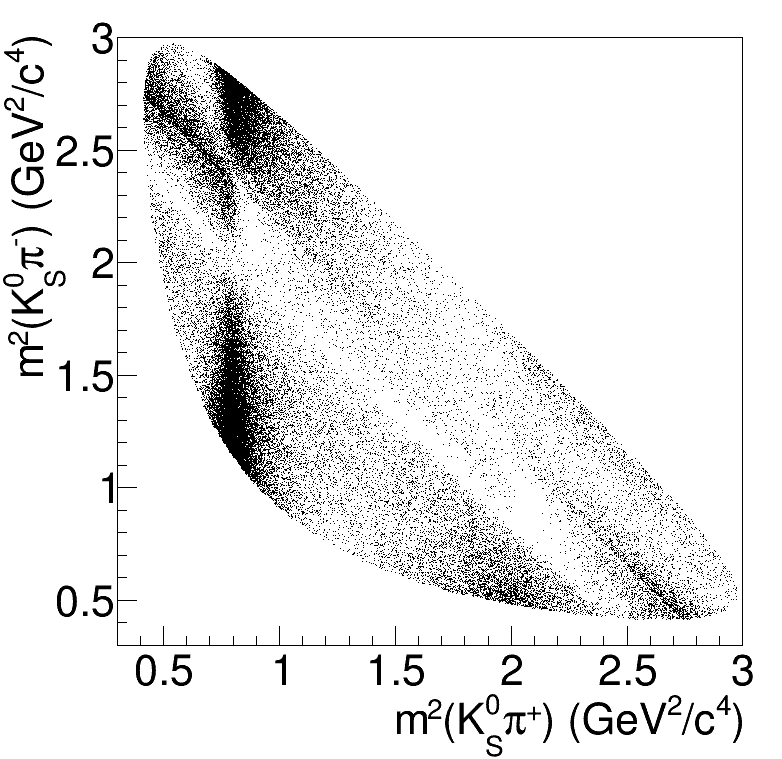
\includegraphics[width=0.85\textwidth]{dp_mc.png}
 \subcaption{}
 \label{fig:dalitz}
\end{minipage}
\begin{minipage}[b]{0.5\textwidth}
 \centering
  \includegraphics[width=0.9\textwidth]{belle_eqdel_bins}
 \subcaption{}
 \label{fig:bd_belle_eqph}
\end{minipage}
 \caption{а) Диаграмма Далица для распада \dbkpp и б)~равномерное по фазе разбиение этой диаграммы, выполненное с помощью модели, полученной с данными детектора \belle.}
 \label{fig:dalitz_plot}
\end{figure}

На рисунке~\ref{fig:dalitz_plot} показано распределение по переменным Далица (диаграмма Далица) для распада \dbkpp и равномерное по фазе разбиение, выполненное на основе полученной в эксперименте \belle модели.  

\paragraph{\boldmath Получение параметров смешивания в когерентных распадах $D$-мезонов.  }  Осцилляции $D$-мезонов описывают \emph{параметры смешивания}
\begin{equation}
 x_D \equiv \frac{\Delta m_D}{\Gamma_D},\quad y_D \equiv \frac{\Delta\Gamma_D}{2\Gamma_D},
\end{equation}
где $\Delta m_D$ ($\Delta\Gamma_D$) обозначает разность масс (ширин) массовых состояний нейтральных $D$-мезонов и $\Gamma_D$ обозначает полусумму ширин этих состояний.  Параметры смешивания малы $x_D\sim y_D\sim 10^{-2}$, поэтому мы всюду используем разложение в ряд по этим параметрам.

Параметры смешивания могут быть получены модельно-независимым образом в когерентных распадах пар $\dn\dnbar$, находящихся в симметричном по перестановке состоянии с $\cconj=+1$.\footnote{Для наглядности мы предполагаем сохранение \cpconj-симметрии в смешивании $D$-мезонов, хотя обсуждаемые ниже методы позволяют получить параметры \cpconj-нарушения в смешивании вместе с параметрами смешивания $D$-мезонов, если рассмотреть более общий формализм.}  Такие пары можно получить в распадах $\ep\to \dn\dbar{}^{*0}$, $\dbar{}^{*0}\to\dnbar\gamma$.  Пусть один из $D$-мезонов такой пары переходит в состояние~\kspp.  Вероятность попадания в область диаграммы Далица с индексом~$i$ при этом зависит от типа конечного состояния второго $D$-мезона.  При переходе второго $D$-мезона в \cpconj-собственное состояние с \cpconj-четностью~$\eta_D$ эта вероятность задается выражением
\begin{equation}\label{eq:m_cp_sym}
%  \begin{split}
   \left<M^{\cconj+}_{i,\eta_D}\right> 
   \propto \lbr\ki+\kmi\rbr\lbr1 + 2\eta_D y_D\rbr + 2\ci\sqrt{\ki\kmi}\lbr\eta_D + 2y_D\rbr %\\
   + \oxdydsq.
%  \end{split}
\end{equation}
Соответствующая вероятность при переходе второго $D$-мезона в состояние с определенным ароматом:
\begin{equation}\label{eq:m_flv_sym}
 \left<M^{\cconj+}_{i}\right> 
 \propto \ki + 2\sqrt{\ki\kmi}\lbr y_D\ci+x_D\si\rbr + \oxdydsq.
\end{equation}
Дополнительно можно рассмотреть некогерентный переход \dnbar-мезона, рожденного в процессе $\ep\to D^+D^{-*}$, $D^{-*}\to\dnbar\pi^+$, в состояние \kspp.  Вероятность попадания в область номер $i$ в этом случае:
\begin{equation}\label{eq:kprime}
 \ki^{\prime} \propto \ki + \sqrt{\ki\kmi}\lbr y_D\ci + x_D\si\rbr + \oxdydsq.
\end{equation}
При известных значениях параметров \ki, \ci и \si соотношения~\eqref{eq:m_cp_sym}, \eqref{eq:m_flv_sym} и~\eqref{eq:kprime} позволяют получить параметры смешивания $x_D$ и $y_D$.  

В процессе $\ep\to \dn\dbar{}^{*0}$, $\dbar{}^{*0}\to\dnbar\pin$ образуется когерентная пара~$\dn\dnbar$-мезонов в антисимметричном состоянии с $\cconj=-1$, которое позволяет получить не искаженные смешиванием значения параметров \ki, \ci и \si.  Таким образом, рассматривая совместно распады~$\dbar{}^{*0}\to\dnbar\pin$ и~$\dbar{}^{*0}\to\dnbar\gamma$, можно выполнить измерения, достаточные для получения параметров смешивания $D$-мезонов.  Оптимальной энергией коллайдера для предложенного измерения является~$4.01\gev$, которая находится под порогом рождения~$D^*\dbar{}^*$-пар.  Численные эксперименты показывают, что параметры смешивания могут быть получены с точностью около $10^{-3}$ с данными, соответствующими году работы Чарм-Тау-фабрики со светимостью~$10^{35}\lumi$.

\paragraph{\boldmath Получение параметров смешивания в некогерентных распадах $D$-мезонов с измерением времени распада. } Плотность вероятности перехода \dn-мезона, рожденного в процессе \dstpdpip, в состояние \kspp при условии попадания в $i$-ю область диаграммы Далица:
\begin{equation}\label{eq:kprime-time}
 \ki^{\prime}\lbr t\rbr \propto \dexp\left[ \ki+\sqrt{\ki\kmi}\lbr y_D\ci+x_D\si\rbr\Gamma t+ \oxdydtsq \right].
\end{equation}
%Большое количество нейтральных $D$-мезонов с известным ароматом в момент рождения позволяют получить распады \dstpdpip, в которых знак заряда $\pi$-мезона определяет начальный аромат $D$-мезона.  
Соотношение~\eqref{eq:kprime-time} впервые опубликовано в работе автора диссертации и позволяет получить параметры \ki и параметры смешивания $D$-мезонов во времязависимых измерениях на $B$-фабрике или в эксперименте~\lhcb.  Как уже обсуждалось, значения параметров~\ci и~\si могут быть получены независимо.  Первое получение параметров смешивания описанным методом было выполнено недавно группой~\lhcb. %В этом измерении использованы значения параметров~\ci и~\si, полученные в эксперименте~CLEO.  

\paragraph{\boldmath Влияние смешивания $D$-мезонов и прямого \cpconj-нарушения в распаде \dnkpp на получение угла \gphi. } В перспективе прецизионного модельно-независимого получения угла~\gphi в экспериментах~\belleii и~\lhcb важным вопросом является влияние осцилляций $D$-мезонов на величину~\gphi, полученную модельно-независимом способом в распадах \bdk, \dkpp.  Мы рассмотрели две процедуры: согласно первой процедуре для определения~\gphi используются значения параметров~\ki, \ci и~\si, полученные в когерентных распадах $\dn\dnbar$-пар; вторая процедура отличается от первой тем, что значения параметров~\ki получены в некогерентных распадах, и поэтому искаженны смешиванием (смотрите уравнение~\eqref{eq:kprime}).  %Смешивание $D$-мезонов в обоих процедурах не учитывается при определении величины \gphi.

Смещение \gphi для обоих процедур оценено с помощью численных экспериментов.  Первая процедура (\ki получены в когерентных распадах) приводит к смещению, не превышающему
\begin{equation}
 \delta\gphi^{(\mathrm{max})} = 3\grad\times \frac{\sqrt{x_D^2+y_D^2}}{0.1\rb}\approx 3\grad,\quad \rb = \left|\frac{\mca\lbr B^+\to\dn K^+\rbr}{\mca\lbr B^+\to\dnbar K^+\rbr}\right|.
\end{equation}
При использовании второй процедуры вклад смешивания в вероятность попадания события в область фазового пространства с индексом $i$ дополнительно подавлен фактором порядка \rb и максимальное смещение составляет
\begin{equation}
 \delta\gphi^{(\mathrm{max})} \approx 3\grad\times\rb\times \frac{\sqrt{x_D^2+y_D^2}}{0.1\rb}\approx 0.2\grad.
\end{equation}
Полученные результаты позволяют заключить, что получение параметров~\ki в некогерентных распадах позволяет не учитывать смешивание $D$-мезонов даже при прецизионном модельно-независимом получении~\gphi в эксперименте~\belleii (точность которого может быть близка к $1\grad$).  

%\paragraph{\boldmath Влияние прямого CP-нарушения в распадах D-мезонов на модельно-независимое получение параметра \gphi. } 
С помощью численных экспериментов изучено влияние прямого \cpconj-нарушения в распадах \dnkpp на извлекаемую модельно-независимым способом величину угла~\gphi в распадах~\bdk, \dkpp.  Показано, что смещение~\gphi не превосходит $3\grad$.  Эта величина определяется точностью экспериментального ограничения величины \cpconj-нарушения в распадах \dnkpp, полученного в эксперименте~CDF.  Ожидается, что измерения в экспериментах \lhcb и \belleii позволят значительно уменьшить эту величину, поскольку в СМ не ожидается значимых \cpconj-нарушающих эффектов в распадах $D$-мезонов.  
%Самое точное на данный момент ограничение величины \cpconj-нарушения в распадах \dnkpp получено в эксперименте CDF.  Используя этот результат, посредством численных экспериментом, показано, что смещение наблюдаемой величины угла \gphi при модельно-независимом измерении в распадах \bdk не превосходит $3\grad$.  

Кроме того, показано, что угол \gphi может быть извлечен в распадах \bdk, \dkpp модельно-независимо и без предположения сохранения \cpconj-симметрии в распадах \dnkpp. При этом статистическая чувствительность метода уменьшается незначительно.

\paragraph{\boldmath Модельно-независимое получение угла \pphi. }  Бондарь, Гершон и Кроковный предложили получать угол \pphi в распадах \bdsth, \dbkpp, $h\in\{\pin\eta^{(\prime)},\omega\}$.  Этот метод позволяет разрешить дискретную неопределенность $2\pphi\to\pi-2\pphi$, присущую классическому получению величины \sindbeta в кварковых переходах \btoccs.  Модельно-независимая модификация этого метода, предложенная автором диссертации, приводит к следующему выражению для плотности вероятности распада в~$i$-й области:
\begin{equation}\label{eq:master-formula}
 \begin{split}
  \mcp_i\lbr \dt\rbr &\propto \bexp\left[ 1 + q_B\frac{\ki-\kmi}{\ki+\kmi}\cos\dmdt\right.\\
  &\left.+2q_B\eta_{h^0}(-1)^l\frac{\sqrt{\ki\kmi}}{\ki+\kmi}\sin\dmdt\left(\si\cosdbeta+\ci\sindbeta\right)\right],
 \end{split}
 \end{equation} 
где $\dt$ обозначает разность собственных времен распада сигнального и помечающего $B$-мезонов, $q_B = 1$ ($q_B = -1$) соответствует аромату \bn (\bnbar) сигнального $B$-мезона при $\dt=0$, $\eta_{h^0}$ обозначает \cpconj-четность $h^0$-мезона и $l$ обозначает орбитальный момент $Dh^0$-системы.\footnote{Для распадов \bdstarh, \dbstdbpi, \dbkpp в функции \mcs возникает дополнительный множитель $-1$.}  

{\textbf{Третья глава}} посвящена описанию асимметричного электрон-позитронного ускорителя \kekb и детектора \belle.  В этой главе также обсуждается участие автора в модернизации калориметра детектора \belle для подготовки работы калориметра в эксперименте \belleii.  %Автором был разработан алгоритм измерения параметров 

В {\textbf{четвертой главе}} обсуждается выполненное впервые модельно-независимое измерение угла~\pphi в распадах \bdsth, \dbkpp, $h^0\in\{\pin, \eta, \etap, \omega\}$ (смотрите уравнение~\eqref{eq:master-formula}).  Для измерения использован полный интеграл светимости $711\ifb$, набранный детектором \belle вблизи резонанса \ups, соответствующий $771$ миллионам $\ups\to\bbbar$-событий.  Равномерное по фазе разбиение фазового пространства распада \dnkpp выполнено с помощью модели, полученной ранее в эксперименте~\belle.  Значения параметров \ci и \si для этого разбиения были измерены в эксперименте CLEO.  Значения параметров \ki получены с помощью распадов \bpdpi, \dbkpp.

Процедура анализа событий состоит из нескольких основных этапов.  На первом этапе происходит отбор кандидатов \bdsth с помощью различных кинематических параметров, изучение компонент фона и применение классифицирующих алгоритмов для подавления фона.  На втором этапе для каждого реконструируемого распада определяется доля сигнальных событий посредством анализа двумерного распределения параметров~\de и~\mbc:
\begin{equation}
 \de=E_B^{\cms}-E_{\mathrm{beam}}^{\cms},\quad
 \mbc = \sqrt{\left(E^{\cms}_{\mathrm{beam}}\right)^2-\left(p^{\cms}_{B}\right)^2},
\end{equation}
где $E_B^{\cms}$, $p^{\cms}_{B}$ и $E_{\mathrm{beam}}^{\cms}$ обозначают соответственно энергию $B$-кандидата, импульс $B$-кандидата и энергию пучка в системе центра масс.  Форма сигнального и фонового распределений \de-\mbc изучаются с помощью моделирования.  Заключительный этап анализа состоит анализе распределений по~\dt.  Фоновые \dt-распределения предварительно изучаются с помощью моделирования, а затем уточняются с помощью экспериментальных событий.  Корректность описания фоновых \dt-распределений и функции разрешения по \dt для сигнальных событий контролируется посредством измерения времени жизни \bn-мезона в распадах \bdsth, \dbkpp.  Получение \cpconj-нарушающих параметров осуществляется методом максимального правдоподобия с функцией правдоподобия вида
\begin{equation}\label{eq:lh}
 \mcl(\xi) = \prod\limits_{j=1}^{N}\left[\fsigj\psig\lbr\dtj,\xi\rbr+\lbr 1-\fsigj\rbr\pbkg\lbr\dtj\rbr\right],
\end{equation}
где $N$ обозначает количество отобранных событий, $\psig$ ($\pbkg$) обозначает плотность вероятности для сигнальных (фоновых) событий, $\fsigj$ обозначает вероятность того, что событие $j$ является сигнальным и $\xi\in\{\sindbeta, \cosdbeta, \pphi\}$.  Границы (асимметричных) доверительных интервалов $[\xi_{\mathrm{nl}},\xi_{\mathrm{nr}}]$, соответствующие $n$ стандартным отклонениям, определяются условием
\begin{equation}
 n^{2} = -2\log\lambda(\xi_{\mathrm{nl}}) = -2\log\lambda(\xi_{\mathrm{nr}}),
\end{equation}
где $\xi_{\mathrm{nl}}$ ($\xi_{\mathrm{nr}}$) обозначает левую (правую) границу интервала и $-2\log\lambda(\xi)$ обозначает логарифм отношения вероятностей 
\begin{equation}\label{eq:confidence_intervals}
 -2\log\lambda(\xi)=-2\log\mcl(\xi,\hat{\hat{\vecp}}) + 2\log\mcl(\hat{\xi},\hat{\vecp}).
\end{equation}
Здесь \vecp обозначает множество параметров за исключением~$\xi$, от которых зависит функция правдоподобия~$\mcl$, $\hat{\xi}$ и $\hat{\vecp}$ обозначают значения параметров, минимизирующее функцию правдоподобия, $\hat{\hat{\vecp}}$ обозначает значения параметров, минимизирующие функцию правдоподобия для текущего значения~$\xi$.  На рисунке~\ref{fig:lambda} показаны логарифмы отношения вероятностей для \cpconj-нарушающих параметров.  Следующие значения соответствуют одному стандартному отклонению:
 \begin{equation}\label{eq:final_results}
 \begin{split}
  \sindbeta &= 0.43     \pm 0.27\stat    \pm 0.08    \syst,\\
  \cosdbeta &= 1.06     \pm 0.33\stat^{+0.21}_{-0.15}\syst,\\
  \pphi     &= 11.7\grad\pm 7.8\grad\stat\pm 2.1\grad\syst.
 \end{split}
 \end{equation}

Величина $\sindbeta=0.691\pm0.017$, полученная в кварковых переходах \btoccs, определяет абсолютное значение \cosdbeta, которому соответствуют два значения угла $\pphi\in[0\grad; 180\grad)$.  Представленное в данной работе измерение исключает отрицательное значение \cosdbeta, соответствующее $\pphi = 68.1\grad$, на уровне $5.1$ стандартных отклонений и находится в согласии с положительным значением \cosdbeta, соответствующим значению $\pphi = 21.9\grad$ на уровне $1.3$ стандартных отклонений.  Таким образом, представленное измерение разрешает неопределенность в значении угла \pphi, присущую измерению параметра \sindbeta в переходах \btoccs.

\begin{figure}[htb]
 \begin{minipage}[b]{0.32\textwidth}
  \centering
  \includegraphics[width=\textwidth]{sin_minos_errors_v4}
  \subcaption{}
 \end{minipage}
 \begin{minipage}[b]{0.32\textwidth}
  \centering
  \includegraphics[width=\textwidth]{cos_minos_errors_v4}
  \subcaption{}
 \end{minipage}
 \begin{minipage}[b]{0.32\textwidth}
  \centering
  \includegraphics[width=\textwidth]{phi1_minos_errors_v4}
  \subcaption{}
 \end{minipage}
  \caption{Логарифмы отношений вероятностей~\eqref{eq:confidence_intervals} для а)~\sindbeta, б)~\cosdbeta и в)~\pphi. Квадраты (круги) показывают значения без учета (с учетом) систематических неопределенностей.  Пунктирные и непрерывные линии показывают аппроксимацию полученных значений.  Вертикальные линии показывают значения, соответствующие $\sindbeta=0.691$.  }
  \label{fig:lambda}
\end{figure}

Доминирующие систематические неопределенности представленного измерения имеют статистическую природу.  Основной вклад вносит неопределенность значений параметров~\ci и~\si, полученных в эксперименте~CLEO.  Эти неопределенности могут быть уменьшены с помощью измерений в эксперименте~\besiii.  Другие существенные неопределенности связаны с описанием временного разрешения и распределений по параметрам~\de и~\mbc.  Эти неопределенности зависят от статистики и будут меньше при выполнении измерения в эксперименте~\belleii.  При выполнении описанного анализа, таким образом, показано отсутствие систематических неопределенностей, потенциально ограничивающих точность прецизионного измерения в эксперименте~\belleii.

В {\textbf{заключении}} приведены основные результаты работы и кратко описаны перспективы развития и практической реализации предложенных в работе методов модельно-независимого получения параметров в экспериментах \belleii, \lhcb и на Чарм-Тау-фабрике.


%\newpage
%При использовании пакета \verb!biblatex! список публикаций автора по теме
%диссертации формируется в разделе <<\publications>>\ файла
%\verb!../common/characteristic.tex!  при помощи команды \verb!\nocite! 

%\clearpage
\ifthenelse{\equal{\thebibliosel}{0}}{% Встроенная реализация с загрузкой файла через движок bibtex8
  \renewcommand{\refname}{\large \authorbibtitle}
  \nocite{*}
  \insertbiblioauthor                          % Подключаем Bib-базы
  %\insertbiblioother   % !!! bibtex не умеет работать с несколькими библиографиями !!!
}{% Реализация пакетом biblatex через движок biber
  \insertbiblioauthor                          % Подключаем Bib-базы
%  \insertbiblioother
}

         % Содержание автореферата

\end{document}